\chapter{Tactile Perception}\label{ch:1-tactile-perception}

% problem statement
% involves modeling the contact between the gripper’s tactile sensors and the object, also referred to as Tactile Perception (TP), such that useful data can be extracted for pose estimation.

To solve problem~\ref{prob:2} and~\ref{prob:3}, the \gls{tp} solution to problem~\ref{prob:1} must provide estimates of contact positions, contact normals and skew forces, which is the goal of this chapter. \medskip

To estimate these, different techniques are considered and their performance analyzed, including a \gls{dl} model for simulating realistic tactile skew forces, \gls{rls} for estimating contact normals and the contact positions from the grasping \mat{G}. Contact normals are essential for accurately estimating the pose of an object in contact, while skew forces are critical for predicting the behavior of an object when it is grasped and manipulated by the \gls{sdh}. \medskip

The \gls{rls} methodology is presented for normal estimation \mvar{\vec{n}_{c,i}=\rvec{n_{i,x},n_{i,y},n_{i,z}}^\T\inR{3}}, where \mvar{i\in\{0,1,\dots,n_c \} } and \mvar{n_c} is the number of contact points, followed by the experimental setup and results being presented.\medskip

The technique behind estimating the skew forces \mvar{\vec{f}_{c,i}=\rvec{f_{i,x},f_{i,y},f_{iz}}^\T\inR{3}}, where \mvar{i} goes from \num{1} to \mvar{n_c} as with the contact normals, is presented, which includes the \gls{dl} models architecture as well as the methodology used to test the network. The testing methodology involves the use of various input data, and the output is analyzed for accuracy and realism. The findings are presented and discussed, including the strengths and weaknesses of the network in simulating tactile data. Finally, an assessment is made of the network's ability to produce tactile data that is realistic. \medskip

The contact positions \mvar{\vec{c}_i=\rvec{c_{i,x},c_{i,y},c_{i,z}}^\T\inR{3}}, are found using the grasping matrix \mat{G} provided by~\cite{simulation-of-the-syntouch-biotac-sensor}.\medskip

The skew force and normal estimates are compared to the ones provided by Gazebo's physics engine, and the known \gls{gt} from where conclusions are drawn. Due to a solution to problem~\ref{prob:1} being a requirement for tackling the remaining problems, quantities from the physics engine are applied as enhancements or substitutes for inadequate results from the methods chosen. \medskip

The software used in this chapter is a regression neural network implemented as a Gazebo \texttt{ModelPlugin}~\cite{gazebo-model-plugin} in C++. However, the \gls{dl} model plugin used in the original publication~\cite{simulation-of-the-syntouch-biotac-sensor} has not been updated since \num{2018}, making the code incompatible with the current version of Gazebo API. Moreover, the licensing issues with the files in the \texttt{xmlrpc++} library, which were used for base64 encoding and decoding, necessitated their removal~\cite{base64-encoding-decoding-licensing-issue}. To address these issues, each has been resolved and the plugin has been reorganized and repackaged for compatibility with the current version of Gazebo. The original version of the plugin can be found in~\cite{ruppel-philipp-biotac-gazebo-plugin}, while the fixed and updated version is available at~\cite{melbye-staven-biotac-sim-plugin}. \medskip

The availability of the updated plugin ensures that the project can continue to benefit from the capabilities of the \gls{mlp} based \gls{dl} model for simulating realistic tactile data in the current version of Gazebo.

\section{Methods}\label{sec:1-tactile-perception-method}

\subsection{Recursive Least Squares}\label{sec:1-tactile-perception-recirsive-least-squares}

To use \gls{rls} to estimate the contact normal, the linear velocity \mvar{\hat{\vec{v}}\inR{3}} must be estimated. However, since the contact points may not be consistent across the surface during motion, some points may be missing at certain time steps. To address this issue, the centroid of the contact points \mvar{\bar{\vec{c}}_t\inR{3}} at time \mvar{t} is used as a representative value for each time step. Therefore, the estimated linear velocity can be computed as
%
\begin{equation} \label{eq:v-estimate}
	\hat{\vec{v}} = \frac{\vec{\bar{c}}_{t} - \vec{\bar{c}}_{t-1}}{\Delta t},
\end{equation}

where \mvar{t-1} is the previous time step and \mvar{\Delta t\inR{}} is the time between samples, which in this case is \SI{0.01}{s} as the sampling frequency is \SI{100}{\hertz}. The velocity at the fingertip in contact is then computed as
%
\begin{equation} \label{eq:v-tip-def}
	\vec{v}_{tip} = \hat{\vec{v}} + [\bm{\omega}]_\times \rot[R]{base}{tcp} \vec{r},
\end{equation}

where \mvar{\hat{\vec{v}}} is the estimated linear velocity computed from~\ref{eq:v-estimate}, \mvar{[\bm{\omega}]_\times\inR{3\times 3}} is the skew-symmetric matrix of the angular velocity \mvar{\bm{\omega}\inR{3}} i.e.
%
\begin{equation} \label{eq:skew-symmetric-matrix}
	[\bm{\omega}]_\times = 
	\begin{bmatrix}
		0 & -\omega_z & \omega_y \\ \omega_z & 0 & -\omega_x \\ -\omega_y & \omega_x & 0
	\end{bmatrix} \quad , \quad \bm{\omega} = \rvec{\omega_x, \omega_y, \omega_z}^\T,
\end{equation}

\mvar{\rot[R]{base}{tcp}\inR{3\times 3}} is the rotation matrix from the hand's base to its \gls{tcp}, and \mvar{\vec{r}\inR{3}} is the position of the contact point in the robot's base frame. \medskip

To compute the normal estimate, an initial guess is needed which is computed by
%
\begin{equation} \label{eq:def-n-init}
	\hat{\vec{n}}_{0} = \frac{\hat{\vec{v}}_{1} \times \hat{\vec{v}}_{0}}{\| \hat{\vec{v}}_{1} \times \hat{\vec{v}}_{0} \|_2},
\end{equation}
where \mvar{\hat{\vec{n}}_0\inR{3}} is the initial estimate, \mvar{\hat{\vec{v}}_{0}} and \mvar{\hat{\vec{v}}_{1}} are the linear velocity estimates for time step \num{0} and \num{1}, and \mvar{\|\cdot\|_2} is the \mvar{\ell_2}-norm. \medskip

Using the quantities above, the two main components \mvar{\mat{L}_n^1\inR{3\times 3}} and \mvar{\mat{L}_n^2\inR{3\times 3}} of the desired estimate \mvar{\hat{\vec{n}}_{new}\inR{3}} can be found. Firstly, \mvar{\mat{L}_n^1} is computed as
%
\begin{equation} \label{eq:def-L-n-1}
	\mat{L}_n^1 = \mat{L}_n^1 - \beta \Delta t \mat{L}_n^1 + \frac{\Delta t K_L}{1+\|\vec{v}_{tip}\|_2^2} \vec{v}_{tip} \vec{v}_{tip}^\T,
\end{equation}
with \mvar{\beta\inR{}} being a decay factor, \mvar{K_L\inR{}} is a gain and \mvar{\|\cdot\|_2^2} is the squared \mvar{\ell_2}-norm. \medskip

The second component \mvar{\mat{L}_n^2} is computed by
%
\begin{equation} \label{eq:def-L-2}
	\mat{L}_n^2 = \mat{L}_n^2 - \beta \Delta t \mat{L}_n^2 + \frac{\Delta t K_L}{1+\|\vec{\nabla}\|_2^2} \vec{\nabla} \vec{\nabla}^\T,
\end{equation}

where \mvar{\vec{\nabla}\inR{3}} is the cross product between the contact force \mvar{\vec{f}_c} and the velocity of the tip \mvar{\vec{v}_{tip}} i.e.
%
\begin{equation} \label{eq:def-nabla-rls}
	\vec{\nabla} = \vec{f}_c \times \vec{v}_{tip}.
\end{equation}
Using these components a \gls{pd} controller is used to compute the change in normal \mvar{\dot{\vec{n}}\inR{3}} as 
%
\begin{equation} \label{eq:def-n-dot}
	\dot{\vec{n}} = -\left( \gamma_1 \mat{L}_n^1 + \gamma_2 \mat{L}_n^2 \right)\vec{n},
\end{equation}
where \mvar{\gamma_1\inR{}} is the proportional gain, \mvar{\gamma_2\inR{}} is the derivative gain and \mvar{\vec{n}} is the current estimate. By computing the cross product between \mvar{\vec{n}} and \mvar{\dot{\vec{n}}}, the angular velocity \mvar{\vec{\omega}} is computed
%
\begin{equation} \label{eq:omega-from-n-and-n-dot}
	\vec{\omega} = \vec{n} \times \dot{\vec{n}}.
\end{equation}
Finally, the new normal estimate \mvar{\vec{n}_{new}\inR{3}} can be computed as
%
\begin{equation}
	\vec{n}_{new} = e^{ \left[ \frac{\Delta t }{2} [\vec{\omega}]_\times \right]} \vec{n},
\end{equation}
where \mvar{e^{ \left[ \frac{\Delta t }{2} [\vec{\omega}]_\times \right]}\inR{3\times 3}} is the exponential map of the skew-symmetric matrix which represents the rotation due to the angular velocity over the time step.

\subsection{Network Architecture}\label{sec:1-tactile-perception-method-network-architecture}
% wrap
In~\cite{simulation-of-the-syntouch-biotac-sensor} two different architectures were built, where architecture B is chosen due to its better greater accuracy and lower execution time. The network architecture B can be seen in~\figref{fig:dl-model-tactile-perception}. As inputs, the network takes one contact position \mvar{\vec{c} = \rvec{c_x, c_y,c_z}} along with three skew force vector samples \mvar{\vec{f}_{1}=\rvec{f_{1,x},f_{1,y},f_{1,z}}}, \mvar{\vec{f}_{2}=\rvec{f_{2,x},f_{2,y},f_{2,z}}} and \mvar{\vec{f}_{3}=\rvec{f_{3,x},f_{3,y},f_{3,z}}}, and a temperature input \mvar{T\inR{}}, which makes the input \mvar{\rvec{\vec{c},\vec{f}_1,\vec{f}_2,\vec{f}_3,T}\inR{13}}. The contact point and forces are extracted from Gazebo's physics engine. The outputs of the network are the data format produced by the physical sensor i.e. an output vector of \mvar{\rvec{pdc, pac, tdc, tac, e_1, \dots, e_{19}}\inR{23}}, where \mvar{pdc} is the pressure DC signal, \mvar{pac} is the pressure AC signal, \mvar{tdc} is the temperature DC signal, \mvar{tac} is the temperature AC signal and \mvar{e_1} to \mvar{e_{19}} are the electrode activations. The electrode activations can, according to SynTouch~\cite{biotac-syntouch-manual}, be related to physical quantities by equations which take raw \num{12}-bit integer sensor readings in \mvar{[0,4095]} those values depend on the skin deformation and require individual calibration. This calibration information was not provided by~\cite{simulation-of-the-syntouch-biotac-sensor}.  \medskip

The network architecture consists of four \gls{mlp}s, one for interpreting the position input, one for interpreting the force inputs, one for interpreting the temperature input, and one for combining the interpretations of force and position inputs. \gls{mlp} \num{1}, is responsible for interpreting the position data, consists of four hidden layers, three of which contain \num{512} neurons and uses \gls{relu} as the activation function, while the last uses a linear activation function with \num{64} neurons. The activation functions can be seen marked red if they are \gls{relu}, green if they are linear activation functions and blue if they are sigmoid activation functions in~\figref{fig:dl-model-tactile-perception}. \medskip

\gls{mlp} \num{2} interprets the force inputs but rather than using \num{512}, uses \num{256} for its hidden layers, while still having the linear activation function and the \num{64} neurons in its fourth layer. This \gls{mlp} further differs as the \num{256} neuron layers apply \mvar{\ell_1} bias regularization. The \gls{mlp} \num{3} produces a temperature correction vector using two hidden layers, one with \num{256} neurons and a sigmoid activation function and one with \num{23} neurons and a linear activation function. The last \gls{mlp}, \gls{mlp} \num{4} takes in the element-wise product of \gls{mlp} \num{1} and \num{2}, parses the product through two \num{256} neuron layers with \gls{relu} and one \num{23} neuron layer with a linear activation function.\medskip

The products of \gls{mlp} \num{3} and \num{4} are summed and parsed as the model's output. All of this can be seen in~\figref{fig:dl-model-tactile-perception}.

% which is incorporated to achieve the final output vector. The temperature correction vector, comprising a densely connected layer of 256 neurons with sigmoid activation for smooth temperature regression and a reduction layer with linear activation, set to output size.

% The position and force inputs are handled by two distinct \gls{mlp}s, each comprising three densely connected layers with \gls{relu} activation. To enable accurate differentiation between various areas on the sensor surface, the position column employs \num{512} neurons per layer, whereas the force column employs \num{256} neurons per layer with \mvar{\ell_1} bias regularization. 

% Both columns conclude with a smaller output layer of 64 neurons with linear activation. The outputs of the position and force columns are multiplied together, and the product is processed through two densely connected layers with ReLU activation, each containing 256 neurons. The result is then reduced to output size by a smaller densely connected layer with linear activation. Finally, a temperature correction vector is incorporated to achieve the final output vector. The temperature correction vector is created by a third column, comprising a densely connected layer of 256 neurons with sigmoid activation for smooth temperature regression and a reduction layer with linear activation, set to output size.

% Initially, a densely connected sequential model (referred to as Network A) was developed, with five hidden layers of sizes 1024, 4096, 512, 512, and 512 and a ReLU activation function. Various experiments with different layer sizes, counts, and activation functions were conducted before settling on this configuration.

\begin{figure}[!h]
		\begin{center}
			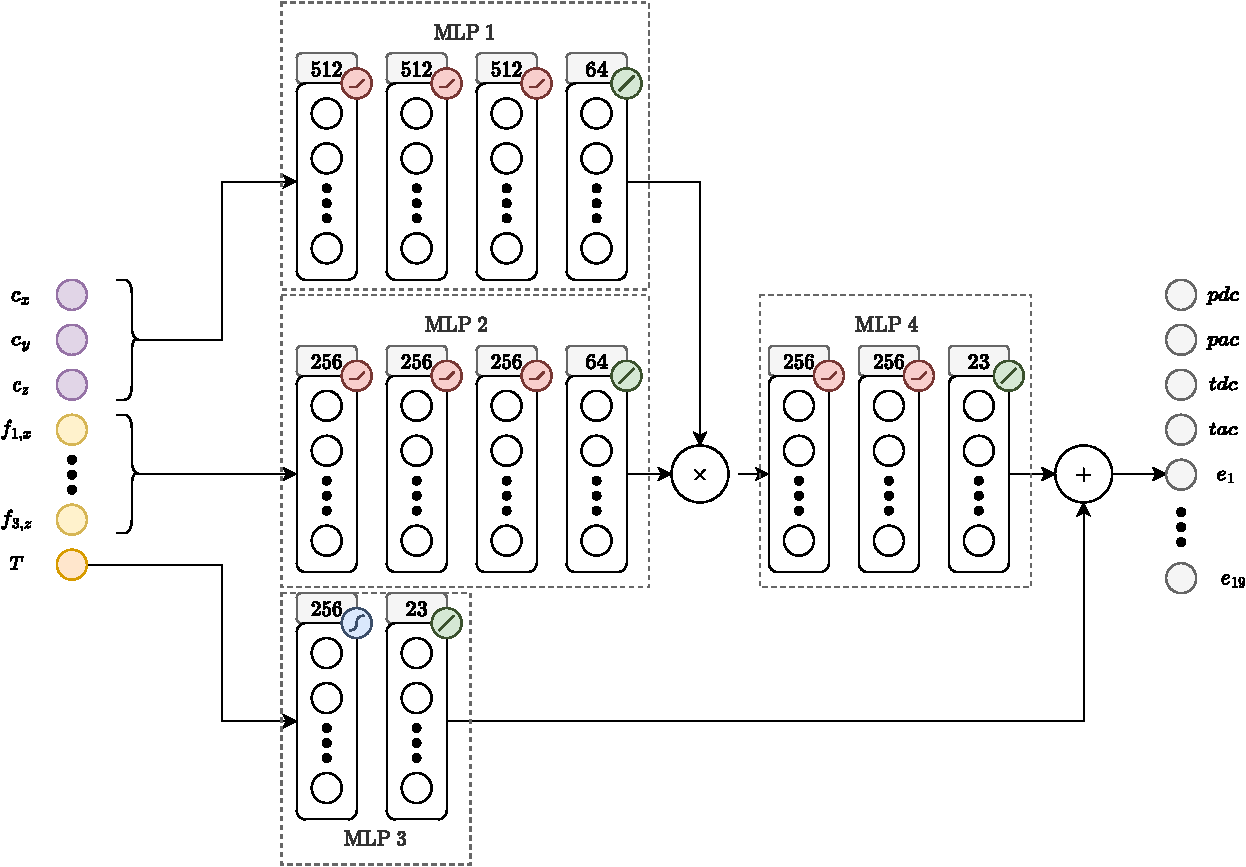
\includegraphics[width=\textwidth]{chapters/1-tactile-perception/fig/drawio/dl-model-tactile-perception-grouping-crop.pdf}
		\end{center}
		\caption{\gls{dl} model B from~\cite{simulation-of-the-syntouch-biotac-sensor}, which also has provided inspiration for this illustration.}
		\label{fig:dl-model-tactile-perception}
\end{figure}

% \newpage

\subsection{Network Training Procedure}\label{sec:1-tactile-perception-method-network-training-procedure}

% The model presented in~\secref{sec:1-tactile-perception-method-network-architecture} was trained using a custom dataset collected by the authors, which led to weights provided in the paper's code that were used rather than retraining the model. The dataset \mat{D} contains \mvar{N_{dp} = \num{300 000}} tactile sensor readings, consisting of the complete BioTac sensor data as well as the applied reference forces and contact points. Meaning \mat{D} is structured as

The model described in~\secref{sec:1-tactile-perception-method-network-architecture} was trained using a custom dataset collected by the authors. Instead of retraining the model, the provided weights in the paper's code were utilized. The dataset, denoted as \mat{D}, comprises \mvar{N_{dp} = 300,000} readings from tactile sensors. It includes complete BioTac sensor data, as well as the corresponding reference forces and contact points. The structure of dataset \mat{D} can be represented as follows
%
\begin{equation} \label{eq:dl-data-matrix}
	\mat{D} =
	\left[\begin{array}{@{}c|cccccccccccccc@{}}
		0       & pcd & pac & tdc & tac & e_{1} & \cdots & e_{19} & f_{1,x} & \cdots & f_{3,z} & c_x & c_y & c_z \\
		1       & pcd & pac & tdc & tac & e_{1} & \cdots & e_{19} & f_{1,x} & \cdots & f_{3,z} & c_x & c_y & c_z \\
		\vdots  &  &  &  &  &  &  & \vdots &  &  &  &  &  &  \\
		N_{dp}  & pcd & pac & tdc & tac & e_{1} & \cdots & e_{19} & f_{1,x} & \cdots & f_{3,z} & c_x & c_y & c_z
		\end{array}\right] \inR{N_{dp} \times 35}.
\end{equation}

To ensure consistency and avoid bias, all inputs are standardized by normalizing them to have zero mean and unit variance, using the distribution of the captured data. To prevent overfitting and unrealistic reactions to high-frequency inputs that the physics simulator cannot accurately reproduce, the three force vectors are sampled at intervals of \SI{100}{\milli\second}. The BioTac sensor electrode values display a non-linear relationship with device temperature. Attempts to address this issue before inputting the data led to poor performance. Instead, the network was trained to independently compensate for this dependency. During simulation, a constant temperature was assumed, typically corresponding to the average temperature of the room when the data was collected. This temperature was not made public in neither~\cite{biotac-dataset} nor~\cite{simulation-of-the-syntouch-biotac-sensor}. The network generates simulated electrode and pressure signals as outputs but currently does not simulate temperature outputs.\medskip

The forces were collected using a calibrated six-axis force-torque sensor~\cite{ati:-6-axis-force-and-torque-sensor-nano17-series} with a nominal force resolution better than \SI{0.01}{\newton}. The contact position is reconstructed optically using a calibrated HD webcam and two AprilTag markers~\cite{apriltag:-a-robust-and-flexible-visual-fiducial-system}, one mounted on the BioTac and one attached to the probe object. The setup for this can be seen in \figref{fig:biotac-sim-experimental-setup}. Once the contact positions were collected, optimization-based calibrations were made to gain more accurate position estimates. \medskip

The data set has been made publicly available and can be found in~\cite{biotac-dataset}.

\begin{figure}[!h]
	\begin{center}
		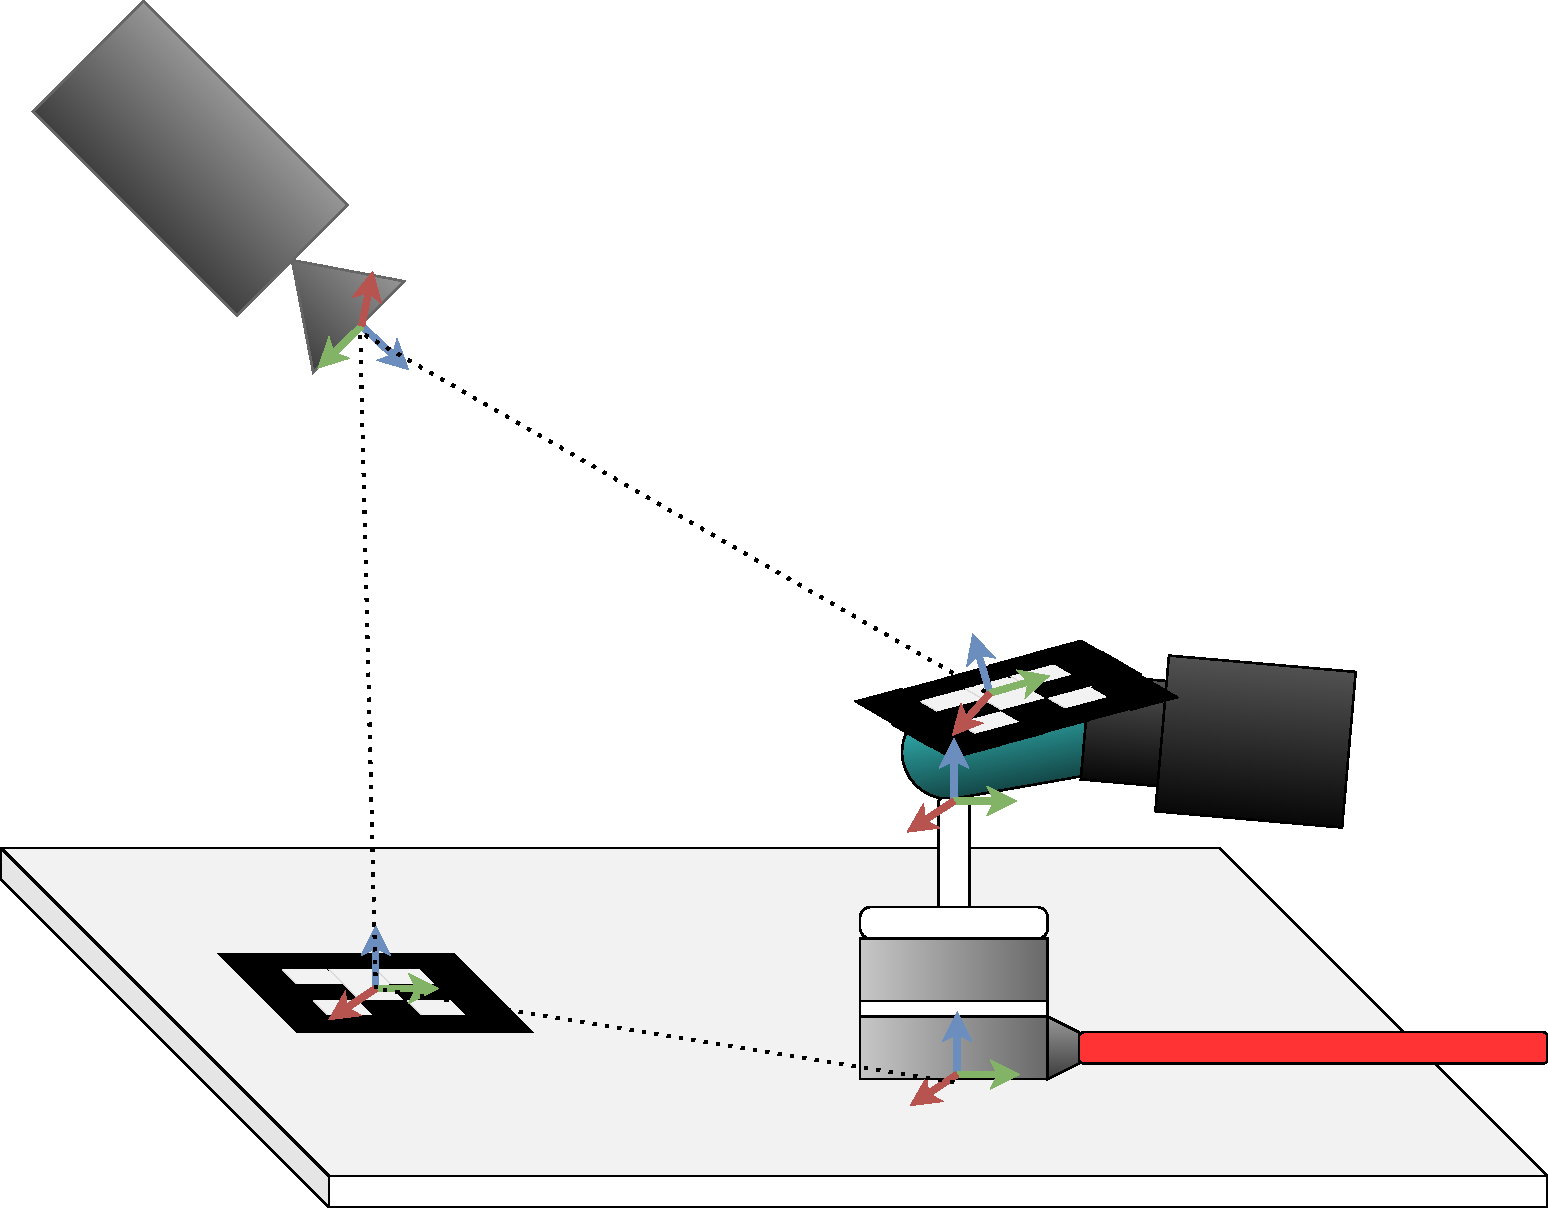
\includegraphics[width=0.6\textwidth]{chapters/1-tactile-perception/fig/drawio/biotac-sim-experimental-setup.pdf}
	\end{center}
	\caption{Experimental setup for gathering data to train \gls{dl} model B, as inspired by~\cite{simulation-of-the-syntouch-biotac-sensor}.}
	\label{fig:biotac-sim-experimental-setup}
\end{figure}
\newpage
\section{Experimental Setup}\label{sec:1-tactile-perception-experimental-setup}

\subsection{Contact Normal Estimation}\label{sec:1-tactile-perception-experimental-setup-contact-normal-estimation}

To test the \gls{rls} method's ability to estimate contact normals the index finger makes contact with a flat surface as shown in~\figref{fig:flat-contact-coor}, through wrist flexion and ulnar deviation a contact path is created as shown in~\figref{fig:2d-projected-contact-path-across-flat-surface}. The motion is done throughout \SI{14}{\second}, and due to a significant presence of noise in the simulated tactile sensors, the contact position data is filtered using a rolling low pass filter with window size \num{100}. The experiment was conducted with the finger on the surface facing \mvar{-\vec{y}}, meaning the \gls{gt} normal is \mvar{\vec{n}_{gt}=\rvec{0,-1,0}} as shown in~\figref{fig:flat-contact-coor}.

\begin{figure}[!h]
	\centering
	\begin{subfigure}[b]{0.48\textwidth}
		\centering
		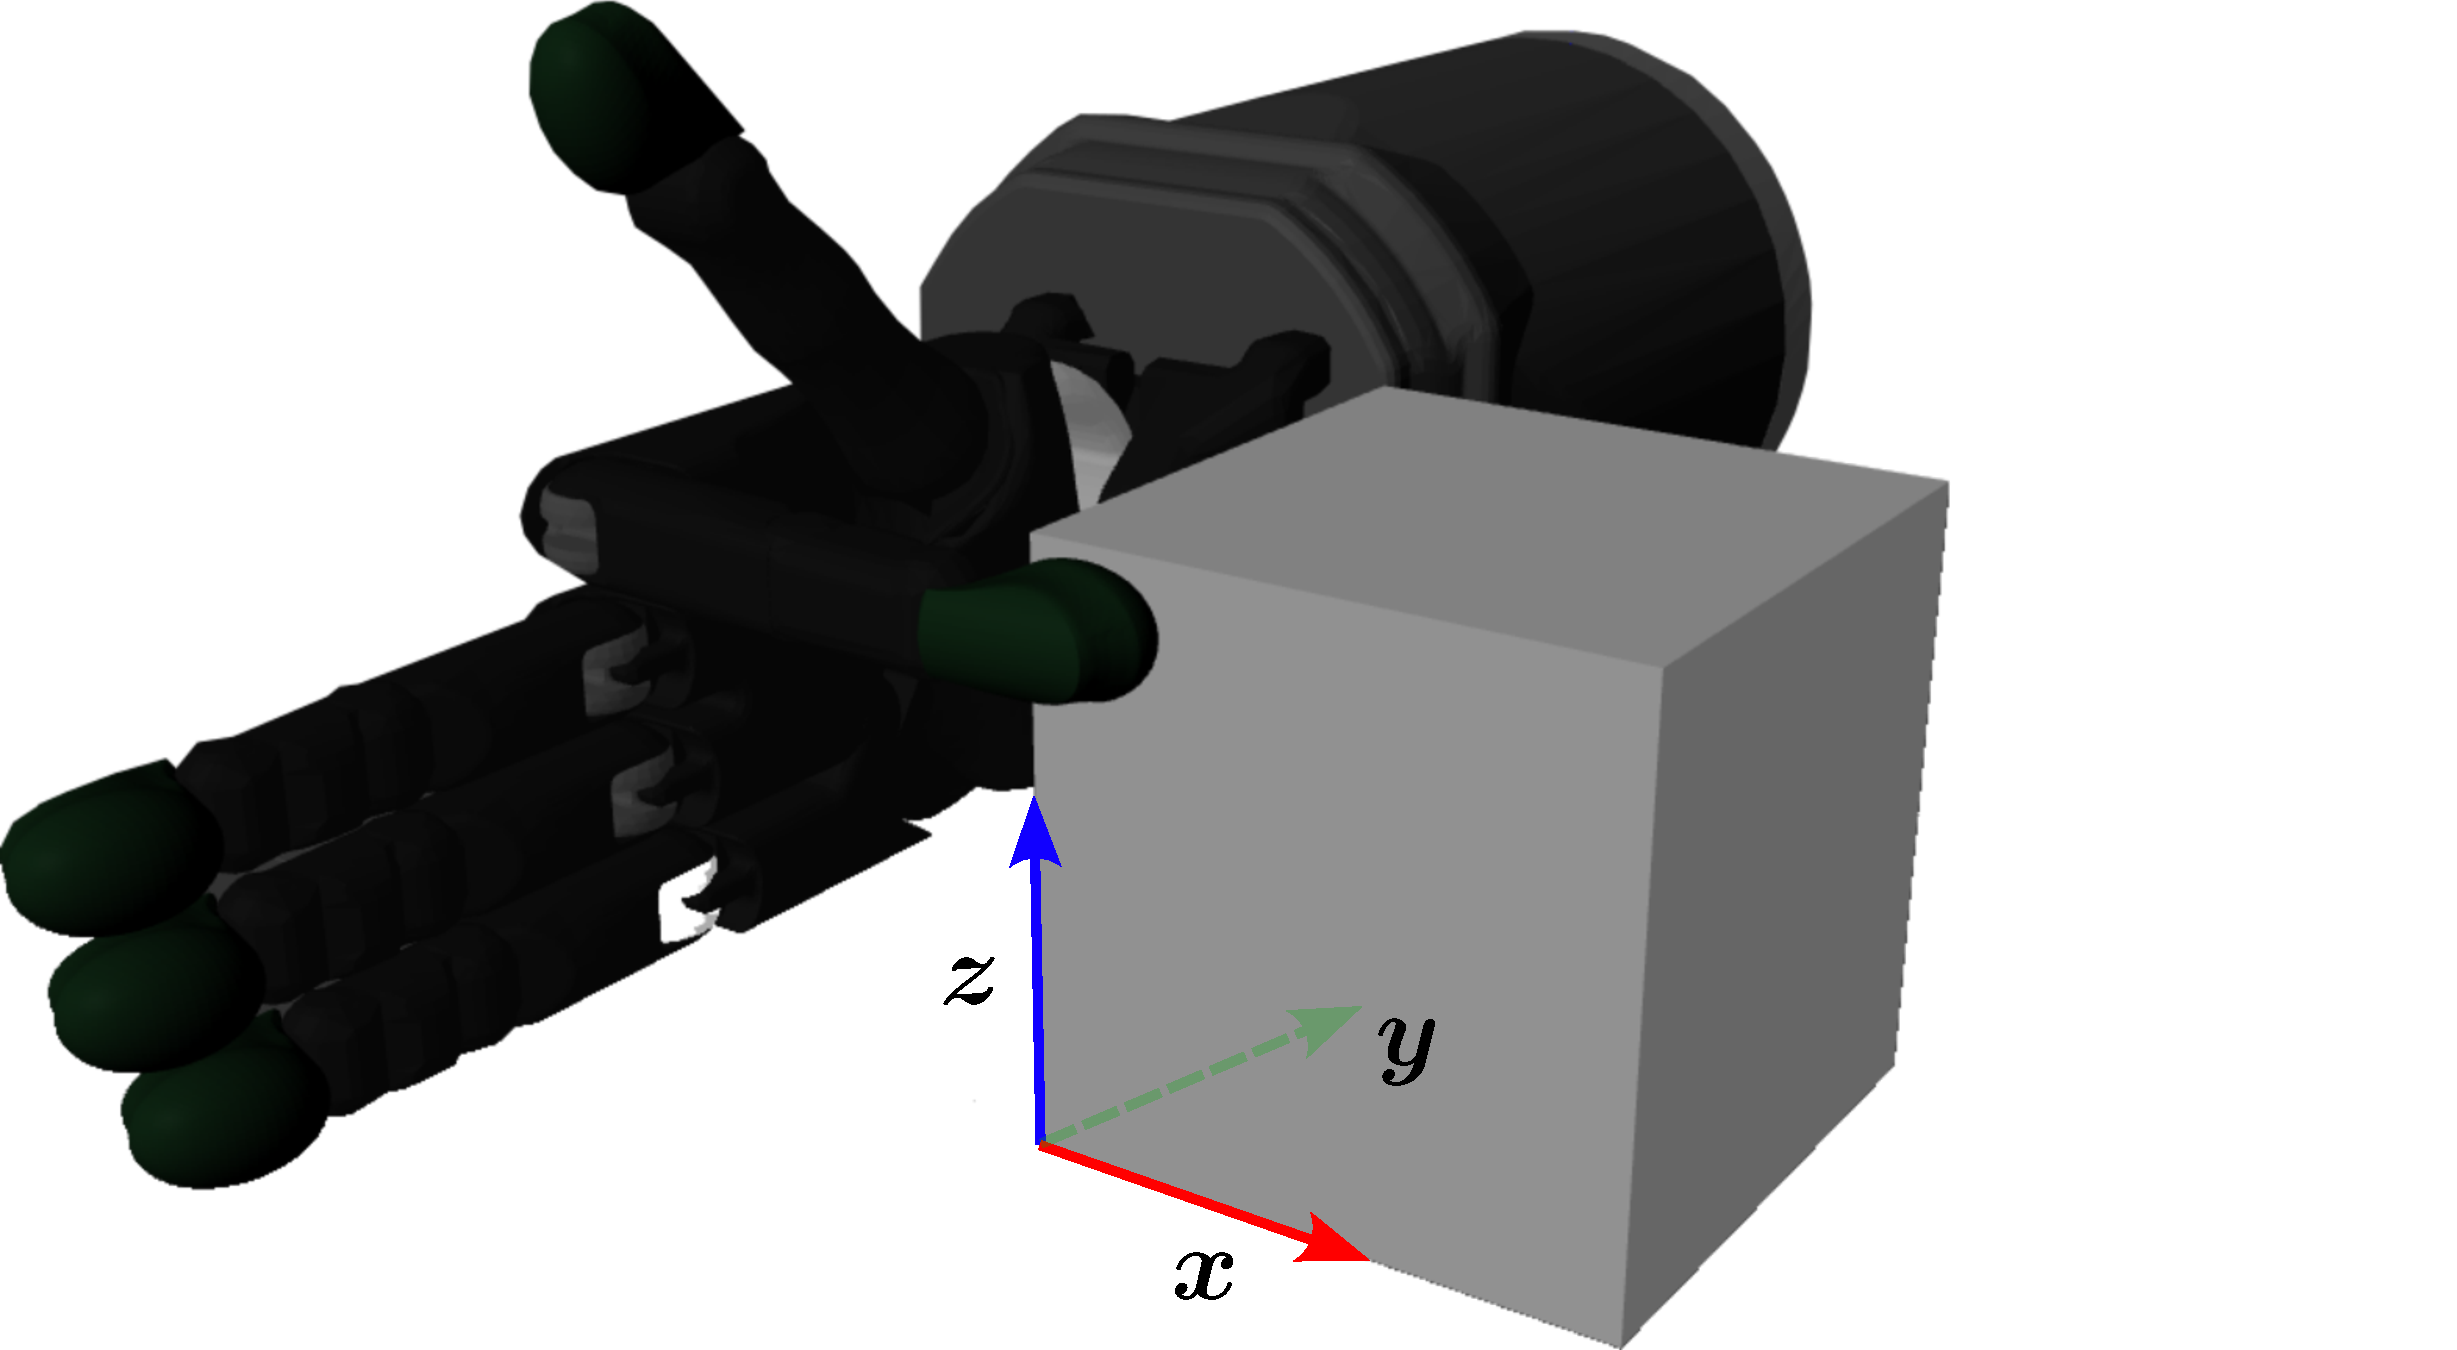
\includegraphics[width=\textwidth]{chapters/1-tactile-perception/fig/inkscape/flat-contact-coor.pdf}
		\caption{Experimental setup for collecting linear velocity data to estimate contact normals using \gls{rls}.}
		\label{fig:flat-contact-coor}
	\end{subfigure}
	\hfill
	\begin{subfigure}[b]{0.48\textwidth}
		\centering
		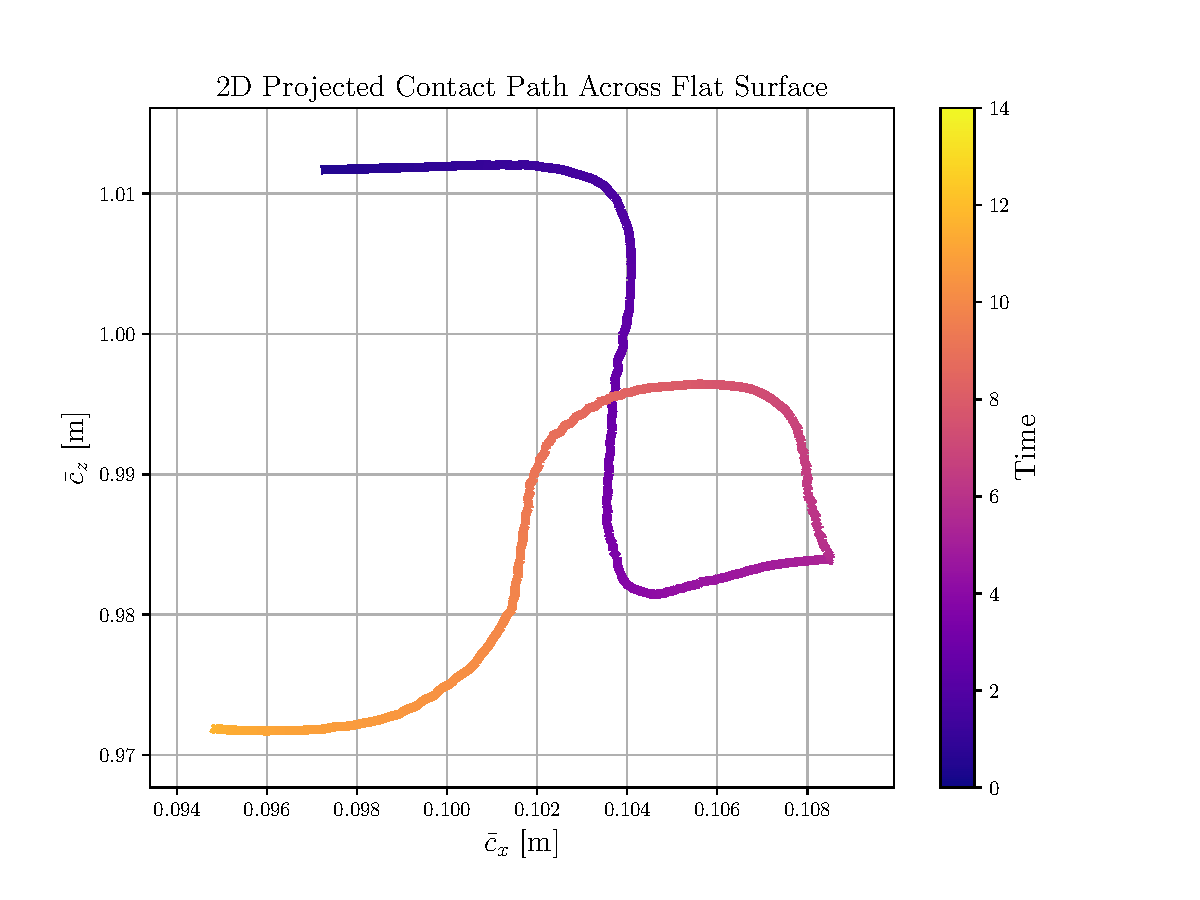
\includegraphics[width=\textwidth]{chapters/1-tactile-perception/fig/matplotlib/2d-projected-contact-path-across-flat-surface.pdf}
		\caption{2D projection of the index finger's path across the cube's flat surface throughout the \SI{14}{\second} data was sampled.}
		\label{fig:2d-projected-contact-path-across-flat-surface}
	\end{subfigure}
		\caption{Experimental setup and index finger's contact path when sampling contact data for normal estimation.}
		\label{fig:experimental-setup-for-normal-estimation}
\end{figure}

\subsection{Skew Force Estimation}\label{sec:1-tactile-perception-experimental-setup-skew-force-estimation}

To test the performance of the \gls{dl} model, four objects surfaces were used with known normals. These can be seen in~\figref{fig:experimental-setup-tactile-perception} as a flat surface, an edge, a smooth surface and a corner.

\begin{figure}[!h]
	\centering
	\begin{subfigure}[b]{0.24\textwidth}
		\centering
		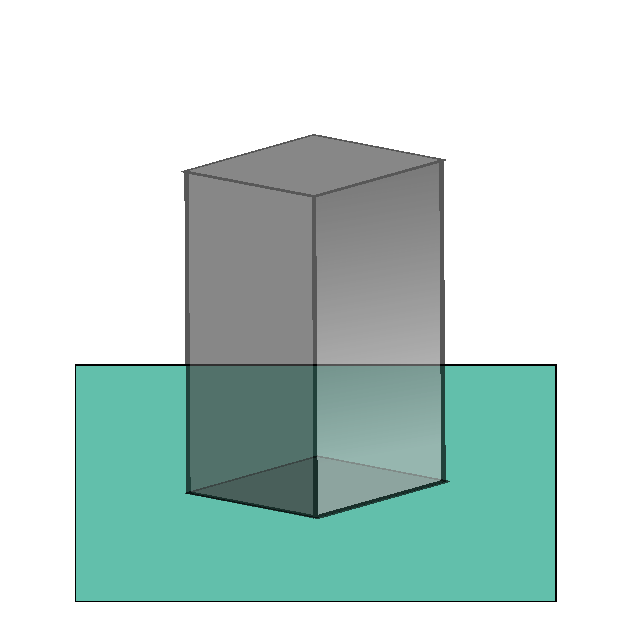
\includegraphics[width=\textwidth]{chapters/1-tactile-perception/fig/inkscape/flat-contact-3d.pdf}
		\caption{Finger in contact with a flat surface.}
		\label{fig:flat-contact}
	\end{subfigure}
	\hfill
	\begin{subfigure}[b]{0.24\textwidth}
		\centering
		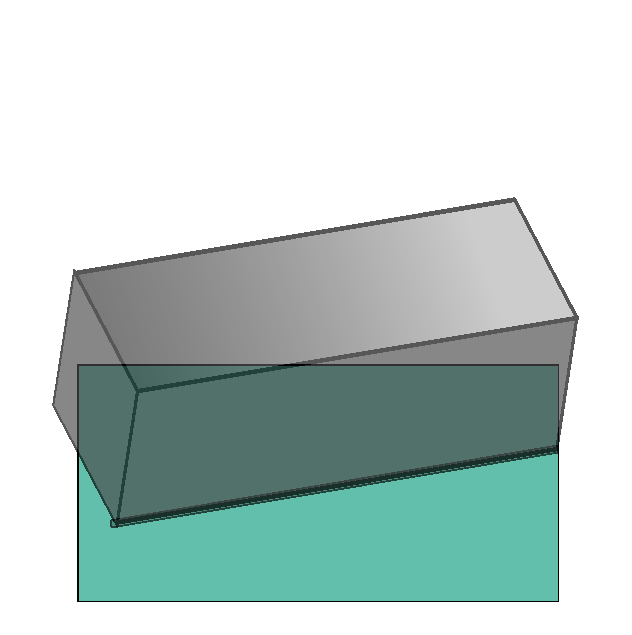
\includegraphics[width=\textwidth]{chapters/1-tactile-perception/fig/inkscape/edge-contact-3d.pdf}
		\caption{Finger in contact with an edge. \newline}
		\label{fig:edge-contact}
	\end{subfigure}
	\hfill
	\begin{subfigure}[b]{0.24\textwidth}
		\centering
		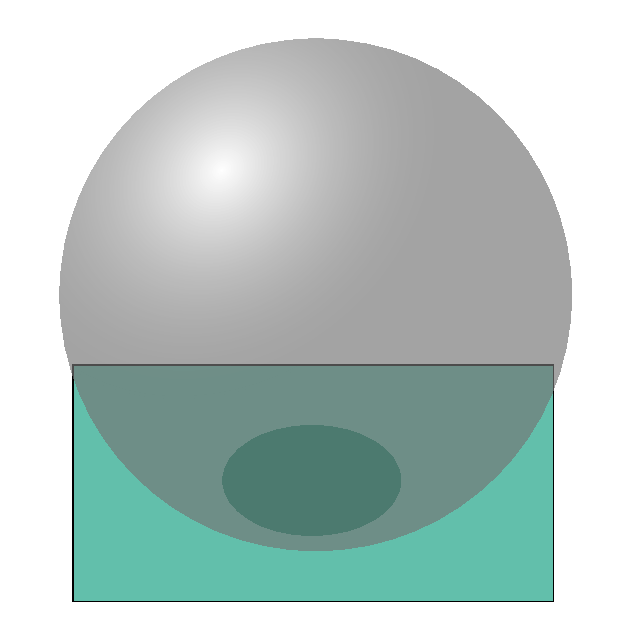
\includegraphics[width=\textwidth]{chapters/1-tactile-perception/fig/inkscape/smooth-contact-3d.pdf}
		\caption{Finger in contact with a smooth surface.}
		\label{fig:smooth-contact}
	\end{subfigure}
	\hfill
	\begin{subfigure}[b]{0.24\textwidth}
		\centering
		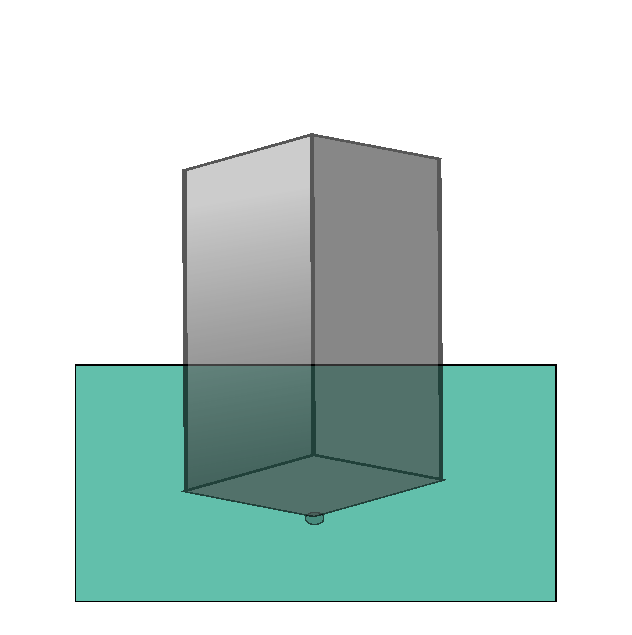
\includegraphics[width=\textwidth]{chapters/1-tactile-perception/fig/inkscape/corner-contact-3d.pdf}
		\caption{Finger in contact with a corner.\newline}
		\label{fig:corner-contact}
	\end{subfigure}
		\caption{The four surfaces used to test the performance of the \gls{dl} model's ability to represent surfaces.}
		\label{fig:experimental-setup-tactile-perception}
\end{figure}

Within the simulation, the index finger is set to make contact with each surface, as shown in~\figref{fig:experimental-setup-tactile-perception-experimental}.
\begin{figure}[!h]
	\centering
	\begin{subfigure}[b]{0.24\textwidth}
		\centering
		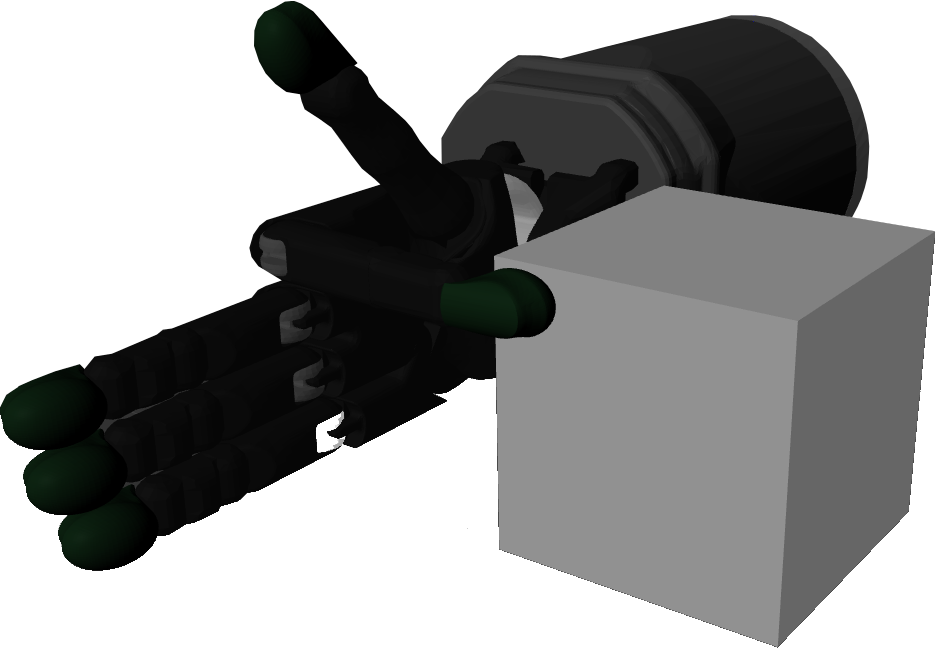
\includegraphics[width=\textwidth]{chapters/1-tactile-perception/fig/screen-shots/flat-contact-crop.png}
		\caption{Simulated index finger in contact with a flat surface.}
		\label{fig:flat-contact-experimental}
	\end{subfigure}
	\hfill
	\begin{subfigure}[b]{0.24\textwidth}
		\centering
		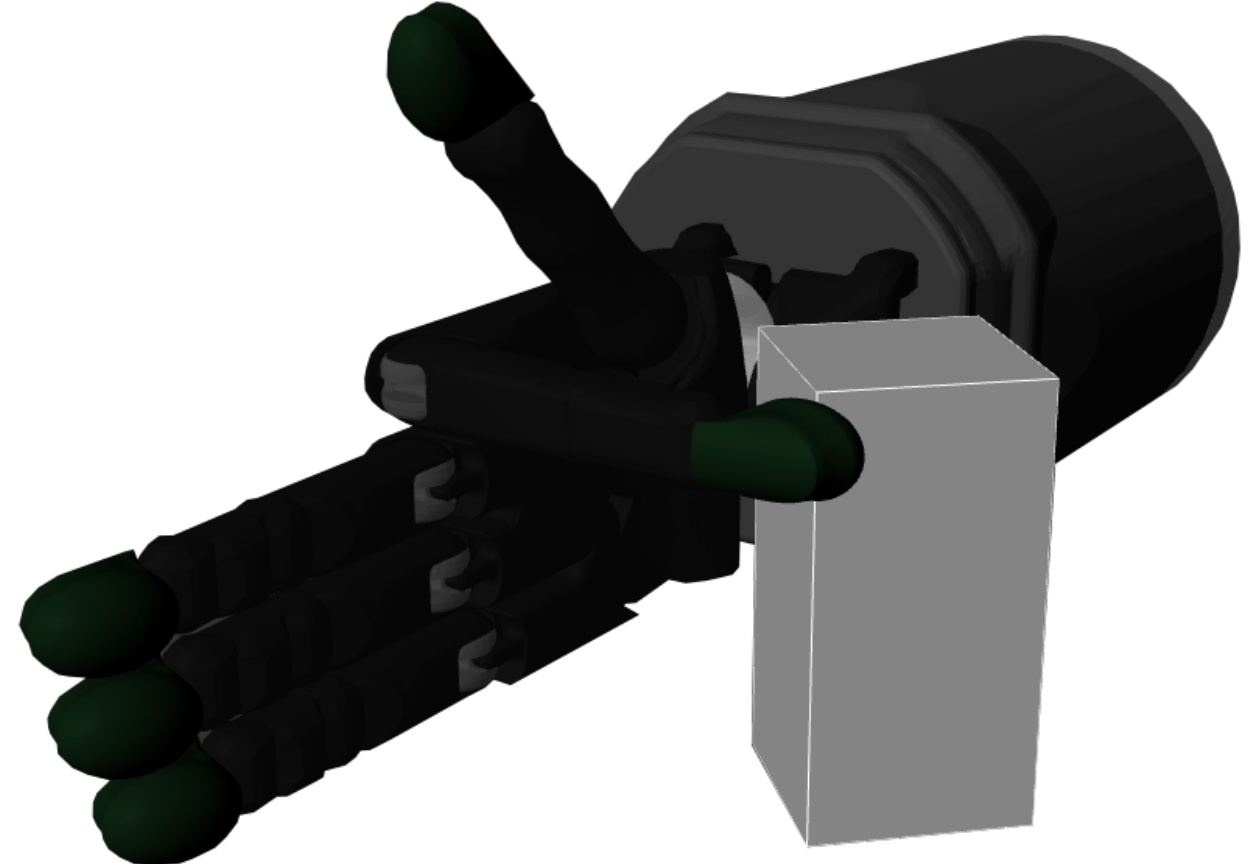
\includegraphics[width=\textwidth]{chapters/1-tactile-perception/fig/screen-shots/edge-contact.png}
		\caption{Simulated index finger in contact with an edge.}
		\label{fig:edge-contact-experimental}
	\end{subfigure}
	\hfill
	\begin{subfigure}[b]{0.24\textwidth}
		\centering
		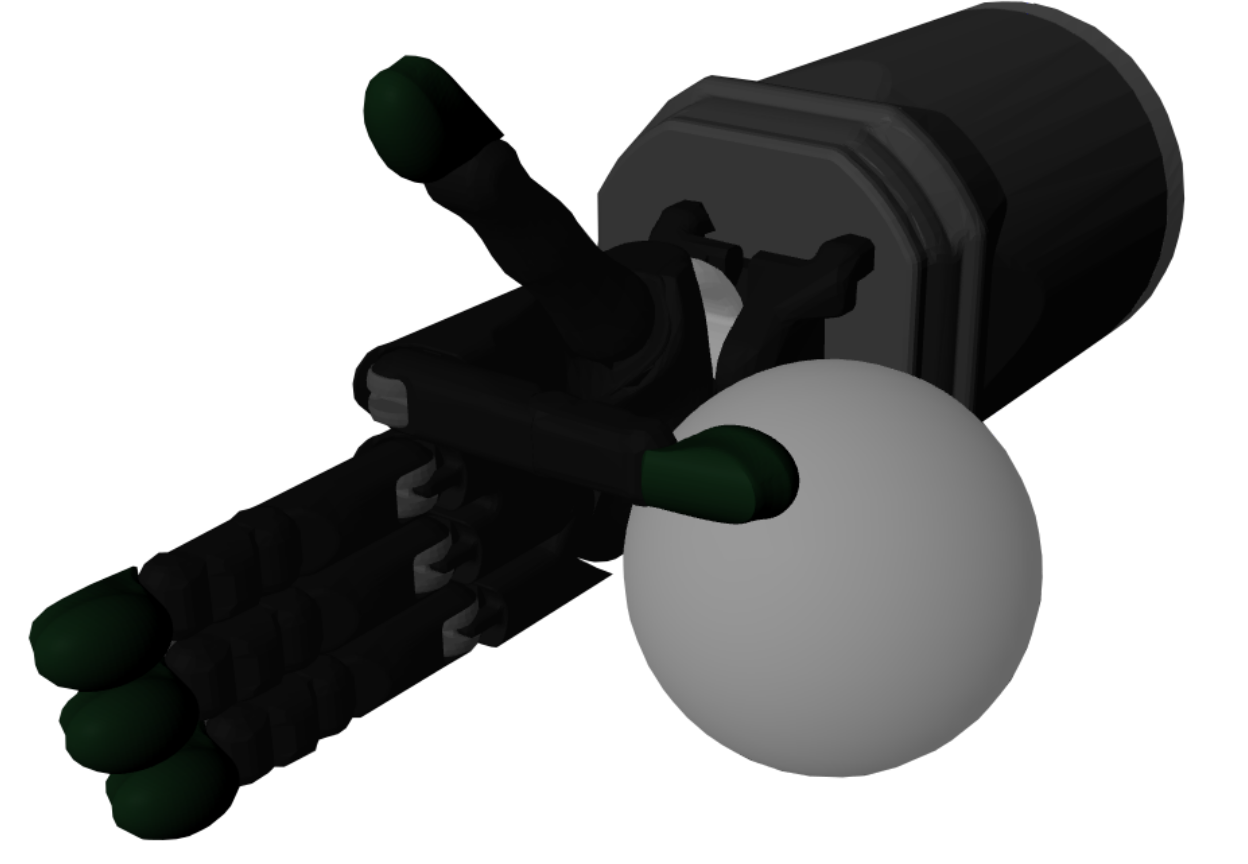
\includegraphics[width=\textwidth]{chapters/1-tactile-perception/fig/screen-shots/smooth-contact.png}
		\caption{simulated index finger in contact with a smooth surface.}
		\label{fig:smooth-contact-experimental}
	\end{subfigure}
	\hfill
	\begin{subfigure}[b]{0.24\textwidth}
		\centering
		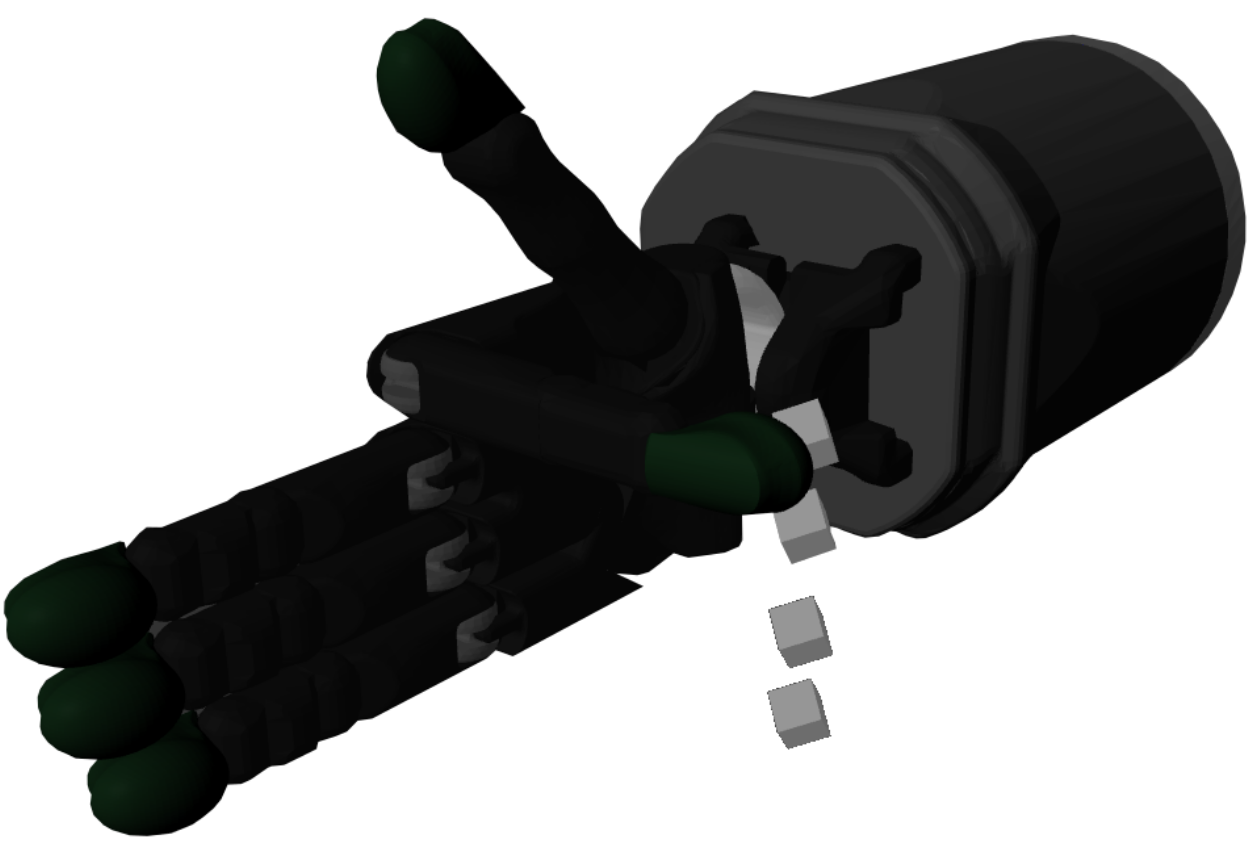
\includegraphics[width=\textwidth]{chapters/1-tactile-perception/fig/screen-shots/corner-contact.png}
		\caption{Simulated index finger in contact with a corner}
		\label{fig:corner-contact-experimental}
	\end{subfigure}
		\caption{The simulated \gls{sdh} in contact with the four surfaces used to test the performance of the \gls{dl} model's ability to represent surfaces. In each case, the contact is made by the index finger.}
		\label{fig:experimental-setup-tactile-perception-experimental}
\end{figure}

When contact is made the inputs and outputs of the \gls{dl} model are recorded over \SI{30}{\second}, which with a sampling frequency of \SI{100}{\hertz} results in \num{3 000} samples. As inputs are collected, the contact positions and forces are given by Gazebo in \robframe{W}, which then is transformed into the contact frame \robframe{C} using the grasping matrix \mat{G}. Due to contact data in Gazebo being prone to noise, an exponential decay filter is additionally applied.

% ground truth vectors presented on figures and how errors were computed

% holding bunny, and logging forces. Forces compared to the theoretical ideal.

% as a solution, one can train an object detection NN for converting tactile data into contact points and normals.
\newpage
\section{Results}\label{sec:1-tactile-perception-results}

\subsection{Contact Normals}\label{sec:1-tactile-perception-results-contact-normals}

Upon estimating the linear velocities~\figref{fig:linear-velocity-finger-in-contact-with-flat-surface} was produced, which shows the three velocity components. Due to the great presence of noise, a rolling low pass filter was applied with a window size of \num{100}. As one would expect \mvar{v_y} shows a negligible magnitude. \medskip

\begin{figure}[!h]
	\begin{center}
		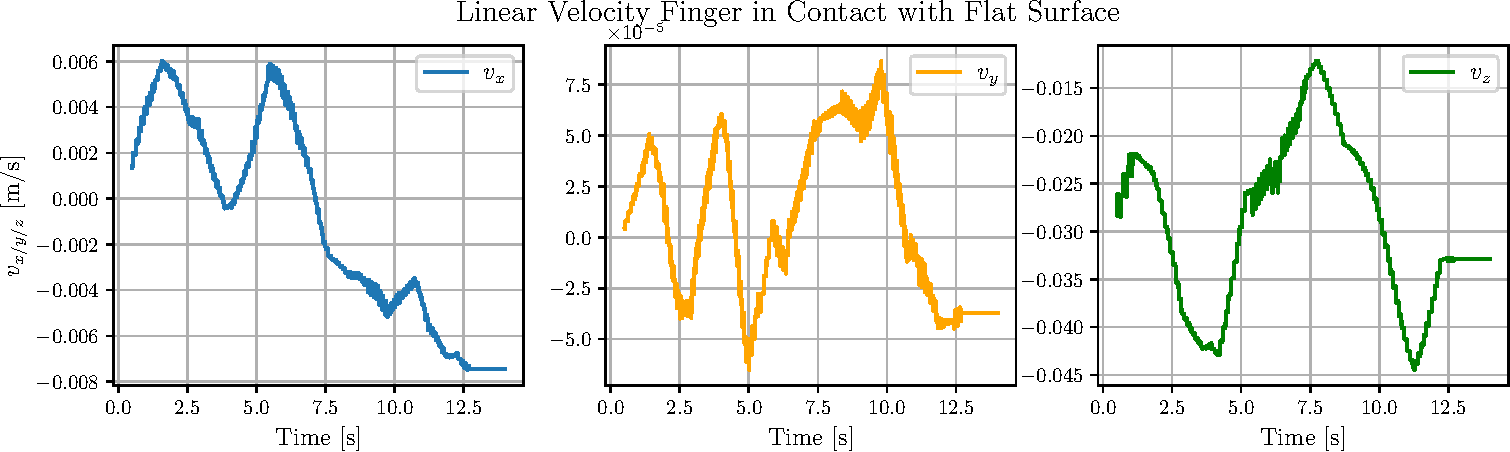
\includegraphics[width=\textwidth]{chapters/1-tactile-perception/fig/matplotlib/linear-velocity-finger-in-contact-with-flat-surface.pdf}
	\end{center}
	\caption{Linear velocities of the contact points when the index finger moves across a flat surface as shown in~\figref{fig:flat-contact-coor}.}
	\label{fig:linear-velocity-finger-in-contact-with-flat-surface}
\end{figure}

Based on these velocities the contact normals were estimated using \gls{rls}, which resulted in~\figref{fig:contact-normal-estimates}, showing great consistency and accuracy over the \SI{14}{\second} the experiment was performed.

\begin{figure}[!h]
	\begin{center}
		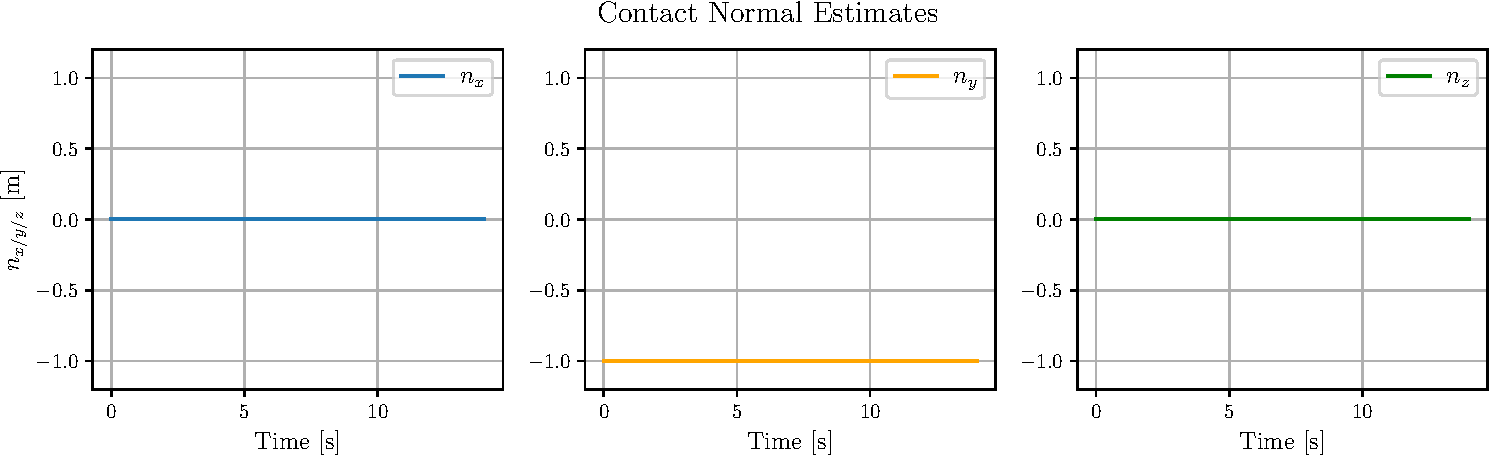
\includegraphics[width=\textwidth]{chapters/1-tactile-perception/fig/matplotlib/contact-normal-estimates.pdf}
	\end{center}
	\caption{The normal estimates across time as the experiment was executed.}
	\label{fig:contact-normal-estimates}
\end{figure}

\subsection{Skew Forces} \label{sec:1-tactile-perception-results-skew-forces}

After executing the \gls{dl} model on all cases, the resulting simulated electrode activations were discovered to be infinite. Consequently, efforts were made to address this issue. It was determined that the model does not include layer-wise normalization to establish limits on feature responses. The addition of this normalization procedure resulted in the network outputting values within the expected range.~\figref{fig:simulated-electrode-distribution} shows a 3D plot of the electrode activations after layer-wise normalization, while~\figref{fig:electrode-map} shows a 2D projection of the finger tip with its electrodes labeled.

\begin{figure}[!h]
	\centering
	\begin{subfigure}[b]{0.48\textwidth}
		\centering
		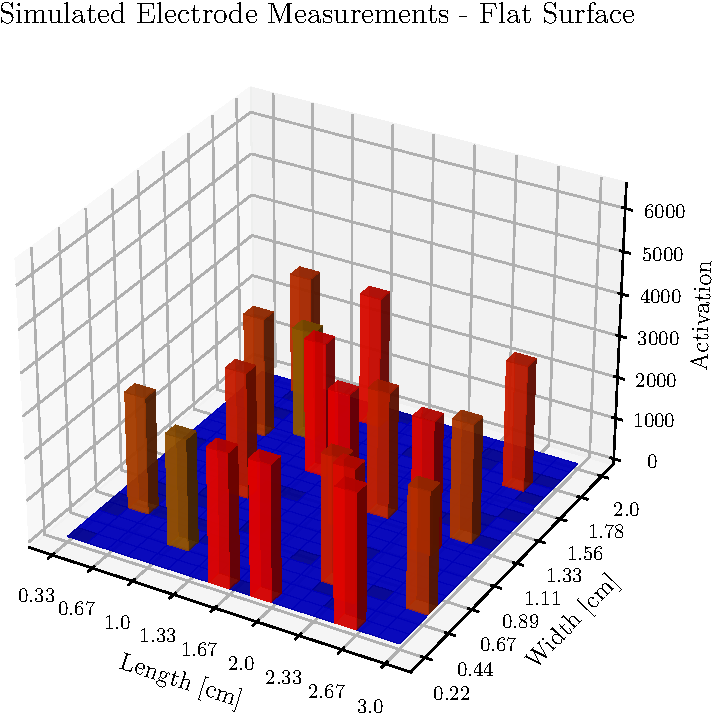
\includegraphics[width=\textwidth]{chapters/1-tactile-perception/fig/matplotlib/pressure-distribution.pdf}
		\caption{3D plot of electrode activations when the \gls{sdh}'s index finger makes contact with a flat surface.}
		\label{fig:simulated-electrode-distribution}
	\end{subfigure}
	\hfill
	\begin{subfigure}[b]{0.48\textwidth}
		\centering
		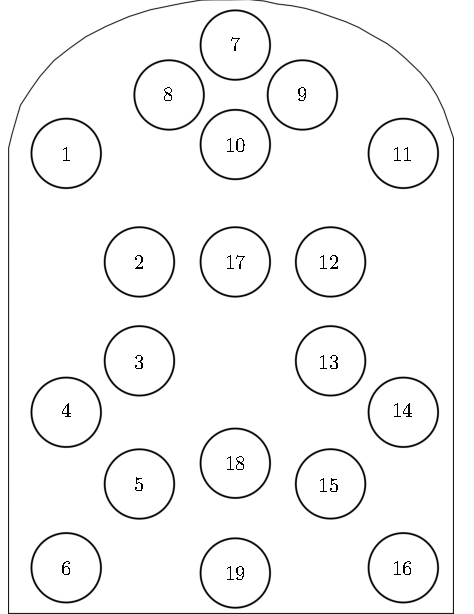
\includegraphics[height=\textwidth]{chapters/1-tactile-perception/fig/drawio/electrode-map.pdf}
		\caption{Map showing a 2D projection of the electrodes' positions and numbers.}
		\label{fig:electrode-map}
	\end{subfigure}
		\caption{3D plot of electrode activations and 2D electrode map with labels.}
		\label{fig:flat-contact-experimental-and-electrode-map}
\end{figure}

\figref{fig:flat-contact-graph} illustrates the inputs and outputs of the \gls{dl} model when the \gls{sdh}'s index finger makes contact with a flat surface. As seen here the output of the model is independent of the input. In an attempt to isolate a potential cause for this behavior, data from the custom data set on which the model had been trained, is applied and similar results were found as seen in~\figref{fig:train-contact-graph}. The missing elements from this graph are value responses from the network of \texttt{inf}, which is a reference to the highest representable value by the system and is therefore not included. \medskip

Due to this independence of input, the electrodes, and by extension the \gls{dl} model is not judged to be able to accurately simulate skew forces for a BioTac sensor in contact. The contact data from the remaining experiments can be found in~\appref{app:tactile-perception-simulated-electrode-activations}, which show a similar pattern.

\begin{figure}[!h]
	\begin{center}
		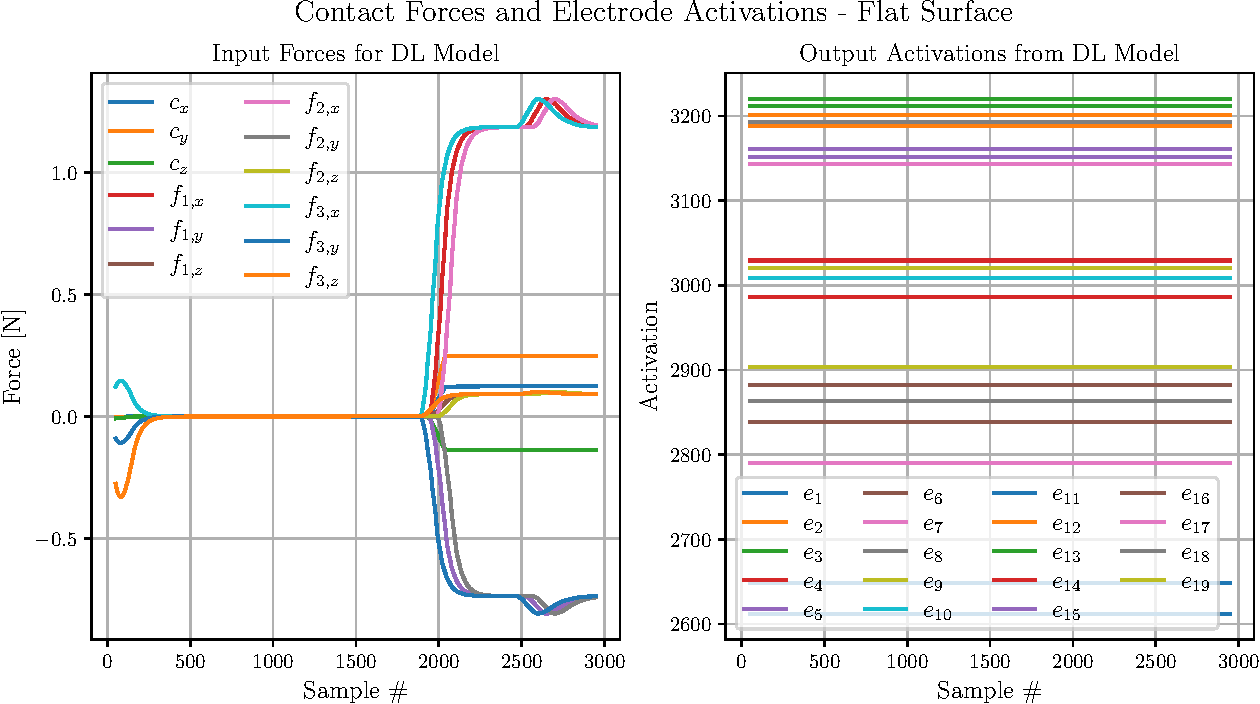
\includegraphics[width=\textwidth]{chapters/1-tactile-perception/fig/matplotlib/flat-contact-graph.pdf}
	\end{center}
	\caption{The simulated tactile electrode activations when the index finger is in contact with a flat surface.}
	\label{fig:flat-contact-graph}
\end{figure}
\begin{figure}[!h]
	\begin{center}
		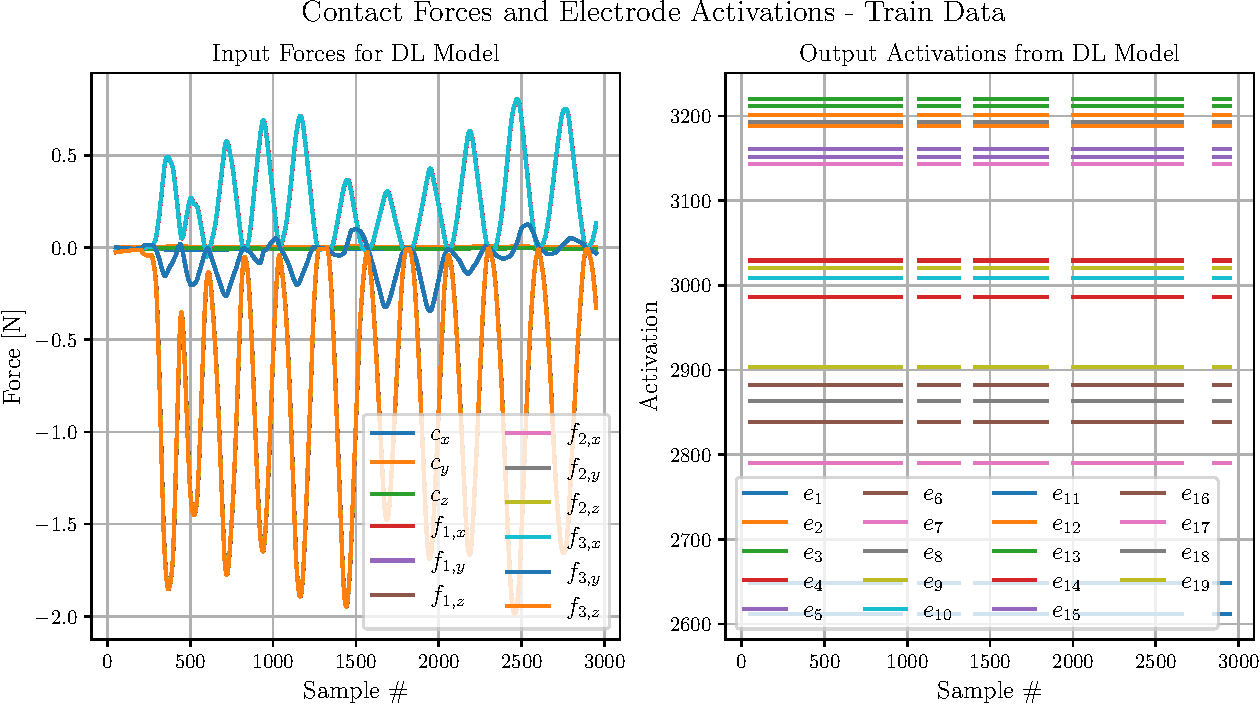
\includegraphics[width=\textwidth]{chapters/1-tactile-perception/fig/matplotlib/train-contact-graph.pdf}
	\end{center}
	\caption{The simulated tactile electrode activations when training data was used as inputs for the \gls{dl} model.}
	\label{fig:train-contact-graph}
\end{figure}

\subsubsection{Contact Positions}

The contact positions were determined by utilizing the grasping matrix \mat{G} and the transformation matrices for each taxel, as provided by~\cite{ruppel-philipp-biotac-gazebo-plugin}. The points in the world frame \robframe{W} were generated using Gazebo's physics engine, and the transformations were applied accordingly. To assess the engine's capability to represent contact points, a 3D mesh of the Stanford bunny~\cite{stanford-bunny} was used. The contact points were recorded during the sampling process, as depicted in~\figref{fig:contact-position-gazebo}. In~\figref{fig:pc-source}, the contact points obtained by moving the fingers across the 3D mesh are shown.~\figref{fig:pc-target} displays the 3D mesh sampled to consist of \num{10 000} points, and~\figref{fig:pc-source-and-target} illustrates both the contact points and the sampled 3D mesh.

% The contact positions were found by applying the grasping matrix \mat{G} and the matrices to transformation to each taxels provided by~\cite{ruppel-philipp-biotac-gazebo-plugin}. The points in \robframe{W} were generated from Gazebo's physics engine, on which the transformations were performed. To test the engine's ability to represent contact points, a 3D mesh of the Stanford bunny~\cite{stanford-bunny} was sampled using the \gls{sdh}, with the contact points being recorded as shown in~\figref{fig:contact-position-gazebo}. Here~\figref{fig:pc-source} shows the contact points sampled from moving the fingers across the 3D mesh,~\figref{fig:pc-target} is the 3D meshed sampled to \num{10 000} points and~\figref{fig:pc-source-and-target}.

\begin{figure}[!h]
	\centering
	\begin{subfigure}[b]{0.3\textwidth}
		\centering
		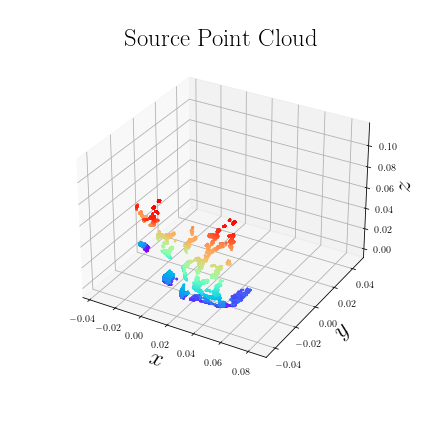
\includegraphics[width=\textwidth]{chapters/1-tactile-perception/fig/matplotlib/pc_source.png}
		\caption{The source \gls{pc} generated from simulated contact points.}
		\label{fig:pc-source}
	\end{subfigure}
	% \hfill
	\begin{subfigure}[b]{0.3\textwidth}
		\centering
		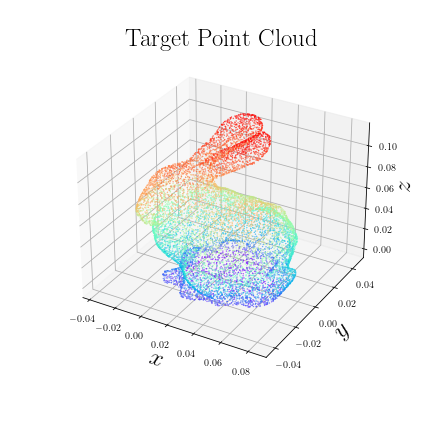
\includegraphics[width=\textwidth]{chapters/1-tactile-perception/fig/matplotlib/pc_target.png}
		\caption{The target \gls{pc} generated by sampling the model mesh with \num{10 000} points.}
		\label{fig:pc-target}
	\end{subfigure}
	% \hfill
	\begin{subfigure}[b]{0.3\textwidth}
		\centering
		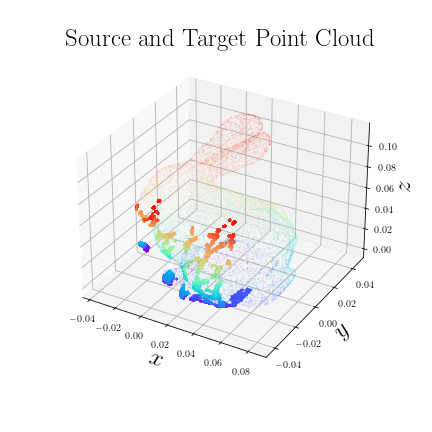
\includegraphics[width=\textwidth]{chapters/1-tactile-perception/fig/matplotlib/pc_source_target.png}
		\caption{The source \gls{pc} overlaid the target \gls{pc}, showing their fit.}
		\label{fig:pc-source-and-target}
	\end{subfigure}
	\caption{3D plots showing the sampled source and target \gls{pc}s along with a plot showing both of them overlaid.}
	\label{fig:contact-position-gazebo}
\end{figure}

\subsection{Physics Engine Comparison}\label{sec:1-tactile-perception-results-gazebo-comparison}

Gazebo's physics engine provides interpretations of contacts for models containing a contact sensor model plugin. The data comes in the form of a \texttt{ContactState} which contain the contact points in \robframe{W}, wrenches, depths and more. As a replacement for the lacking skew forces from the \gls{dl} method and an extension of the normal estimation, Gazebo's physics engine is considered a supplement to the normal estimation and a substitute to \gls{dl} method. The data sampling in this section is restricted to \SI{100}{\hertz} over \SI{100}{\second}. \medskip

The contact forces and torques generated by the engine are shown in~\figref{fig:xy-projected-force-cones} and~\figref{fig:xy-projected-torque-cones}, for the Shadow Dexterous finger's being in contact with an edge. The vectors here are projected into the xy-plane due to the z-component showing a negligible magnitude due to being parallel with the edge, as shown in~\figref{fig:edge-contact-coor}.

\begin{figure}[!h]
	\begin{center}
		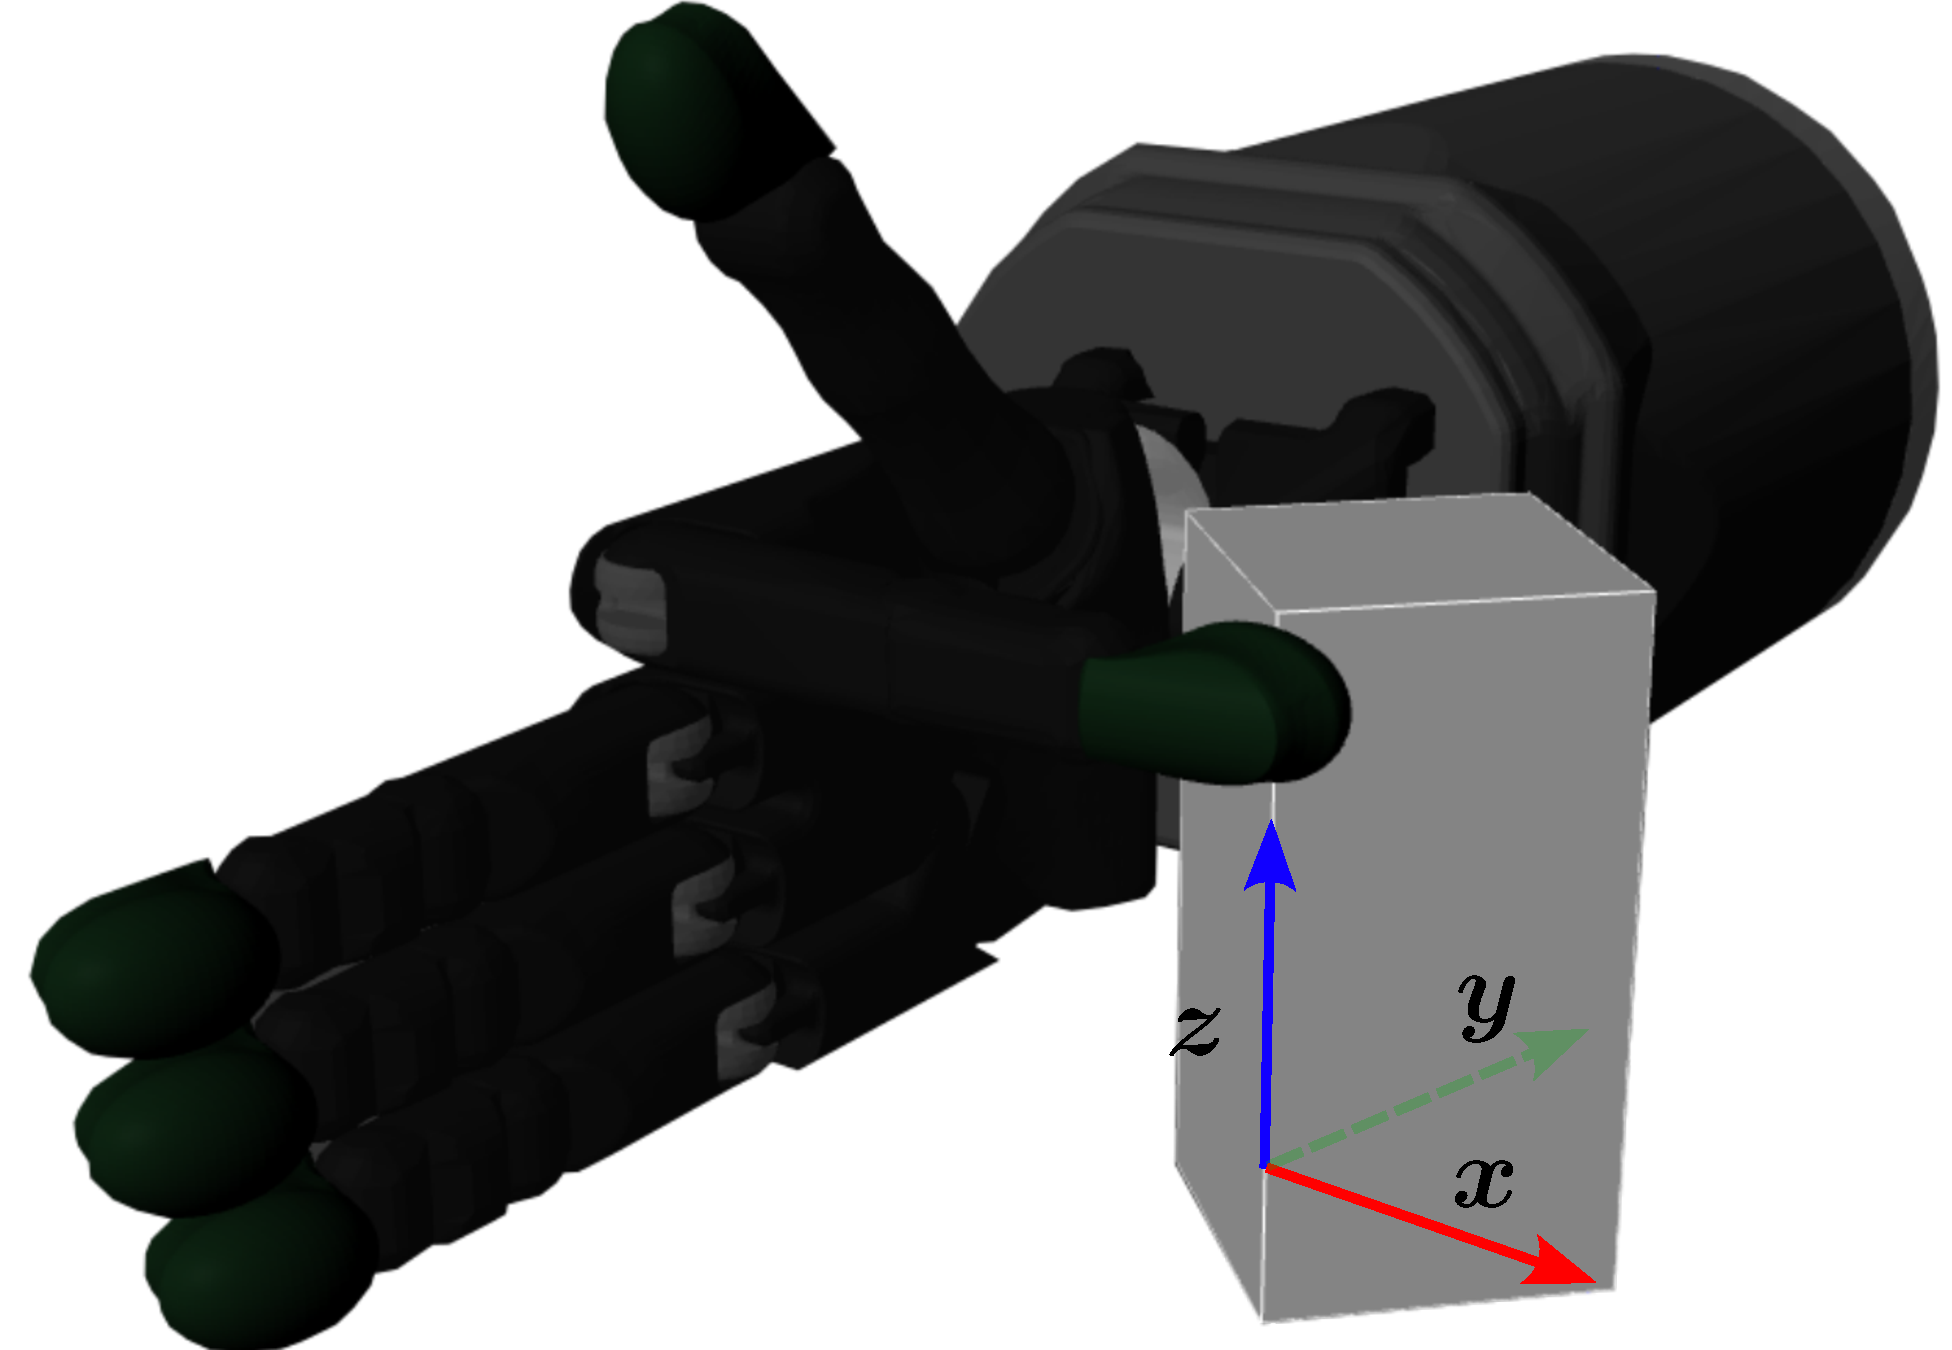
\includegraphics[width=0.5\textwidth]{chapters/1-tactile-perception/fig/edge-contact-coor.pdf}
	\end{center}
	\caption{Simulated \gls{sdh} when in contact with an edge with the coordinate system.}
	\label{fig:edge-contact-coor}
\end{figure}

\begin{figure}[!h]
	\centering
	\begin{subfigure}[b]{0.48\textwidth}
		\centering
		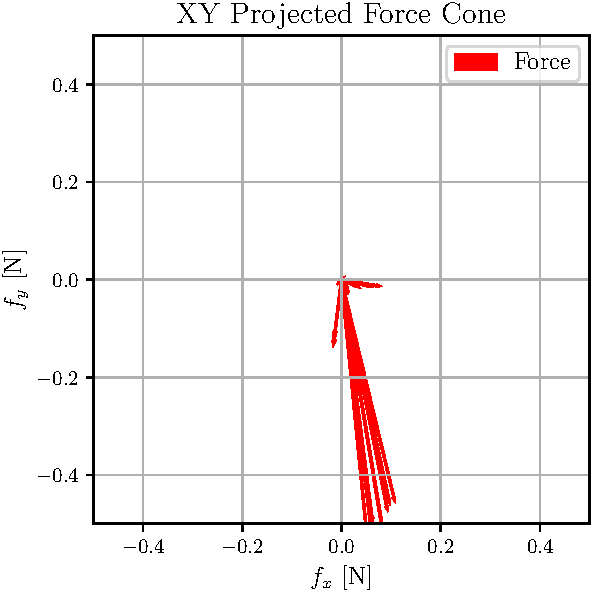
\includegraphics[width=\textwidth]{chapters/1-tactile-perception/fig/matplotlib/xy-projected-force-cones.pdf}
		\caption{XY projected force cone produced by Gazebo's physics engine when the \gls{sdh} is in contact with an edge.}
		\label{fig:xy-projected-force-cones}
	\end{subfigure}
	\hfill
	\begin{subfigure}[b]{0.48\textwidth}
		\centering
		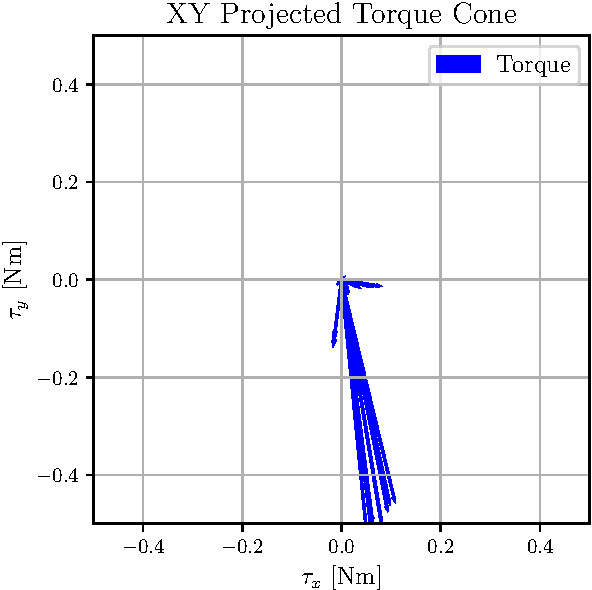
\includegraphics[width=\textwidth]{chapters/1-tactile-perception/fig/matplotlib/xy-projected-torque-cones.pdf}
		\caption{XY projected torque cone produced by Gazebo's physics engine when the \gls{sdh} is in contact with an edge.}
		\label{fig:xy-projected-torque-cones}
	\end{subfigure}
		\caption{XY projected force and torque cones produced by Gazebo's physics engine when the \gls{sdh} is in contact with an edge.}
		\label{fig:xy-projected-force-torque-cones}
\end{figure}

The normals however posed a challenge, as the colliding meshes caused a misinterpretation by the physics engine to produce contact normals which were reflected \SI{180}{\degree}. This can be seen in~\figref{fig:xy-projected-raw-normal-cones}. This was solved by sampling a set of contact normals over \num{10} time steps, reducing the sampling frequency to \SI{10}{\hertz}. These were then clustered using Euclidean clustering with an \mvar{\epsilon} of \SI{1}{\centi\meter} and \num{3} as the minimum number of samples to define a cluster. The centroid of each cluster was then used as the representative and the normal cones shown in~\figref{fig:xy-projected-processed-normal-cones} were achieved.

\begin{figure}[!h]
	\centering
	\begin{subfigure}[b]{0.48\textwidth}
		\centering
		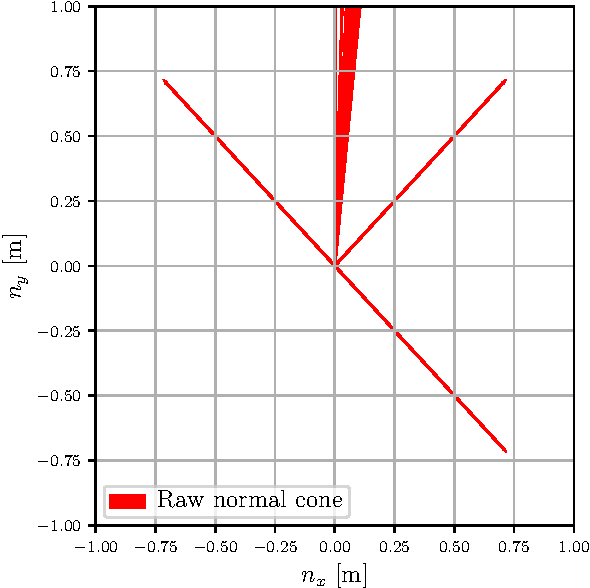
\includegraphics[width=\textwidth]{chapters/1-tactile-perception/fig/matplotlib/xy-projected-raw-normal-cones.pdf}
		\caption{XY projected raw normal cones produced by Gazebo's physics engine when the \gls{sdh} is in contact with an edge.}
		\label{fig:xy-projected-raw-normal-cones}
	\end{subfigure}
	\hfill
	\begin{subfigure}[b]{0.48\textwidth}
		\centering
		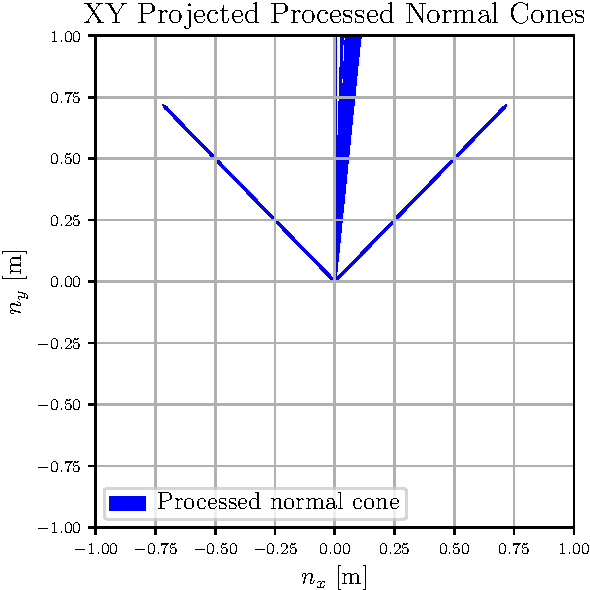
\includegraphics[width=\textwidth]{chapters/1-tactile-perception/fig/matplotlib/xy-projected-processed-normal-cones.pdf}
		\caption{XY projected processed normal cones produced by Gazebo's physics engine when the \gls{sdh} is in contact with an edge.}
		\label{fig:xy-projected-processed-normal-cones}
	\end{subfigure}
		\caption{XY projected raw and processed normal cones produced by Gazebo's physics engine when the \gls{sdh} is in contact with an edge.}
		\label{fig:xy-projected-processed-normal-normal-cones}
\end{figure}

Finally, the angle errors \mvar{\theta_e} between the ground truth normals \mvar{\vec{n}_{gt}} and the simulated contact normals were found for each of the four presented surfaces. The probability distributions over angle errors \mvar{P(\theta_e)} in degrees can be seen in~\figref{fig:histogram-normal-errors}.

\begin{figure}[!h]
	\begin{center}
		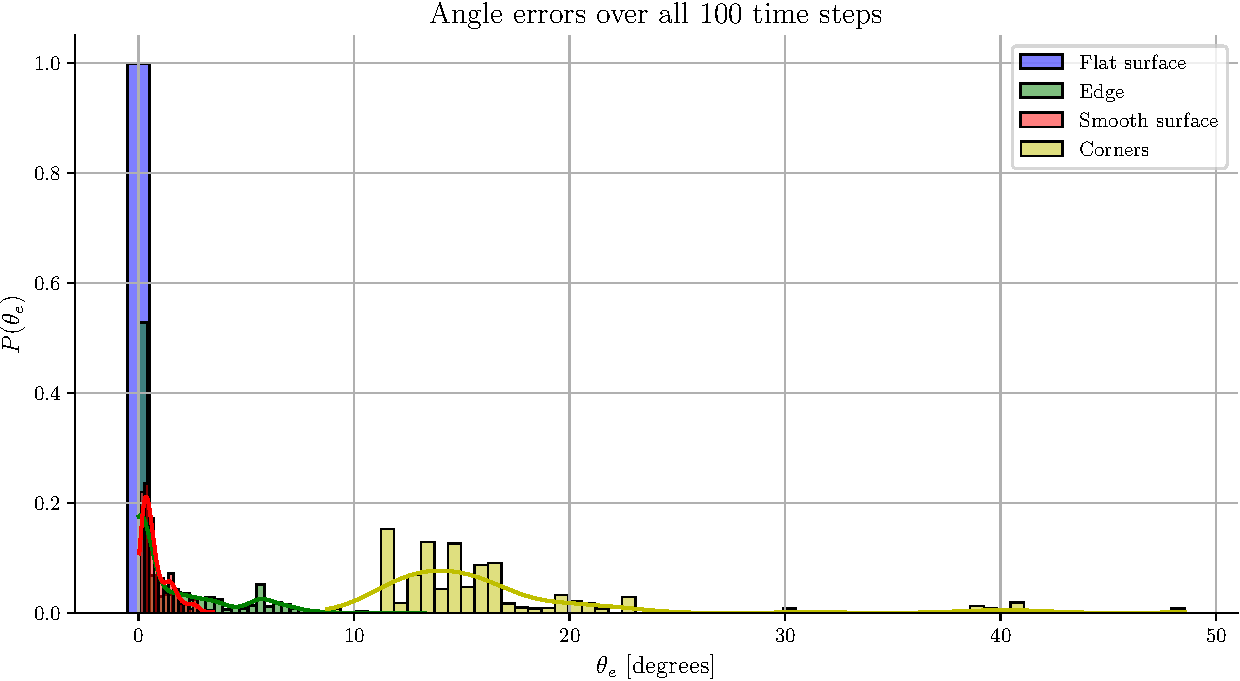
\includegraphics[width=0.9\textwidth]{chapters/1-tactile-perception/fig/matplotlib/histogram-normal-errors.pdf}
	\end{center}
	\caption{Probability distributions \mvar{P(\theta_e)} of the angle error \mvar{\theta_e} between simulated and \gls{gt} contact normals for each tested surface.}
	\label{fig:histogram-normal-errors}
\end{figure}

\newpage
\section{Discussion \& Conclusion}\label{sec:1-tactile-perception-discussion-and-conclusion}


% To solve problem~\ref{prob:2} and~\ref{prob:3}, the \gls{tp} solution to problem~\ref{prob:1} must provide estimates of contact positions, contact normals and skew forces, which is the goal of this chapter. \medskip

In this chapter contact positions, normals and skew forces are successfully estimated or simulated. \medskip

% Finally, the contact positions \mvar{\vec{c}_i=\rvec{c_{i,x},c_{i,y},c_{i,z}}^\T\inR{3}}, which has the same bounds as the skew forces and contact normals are found and evaluated from the grasping matrix \mat{G} provided by~\cite{simulation-of-the-syntouch-biotac-sensor}.\medskip

The contact points have been successfully estimated using simulated contact points and the grasping matrix from~\cite{ruppel-philipp-biotac-gazebo-plugin}. \medskip

% Firstly, the \gls{rls} methodology is presented for normal estimation \mvar{\vec{n}_{c,i}=\rvec{n_{i,x},n_{i,y},n_{i,z}}^\T\inR{3}}, where \mvar{i\in\{0,1,\dots,n_c \} } and \mvar{n_c} is the number of contact points, followed by the experimental setup and results being presented.\medskip

The contact normals were estimated using estimated linear velocities from simulated contact points and the \gls{rls} method. This technique was tested and verified on a flat surface where the results show little error and thus were deemed satisfactory. Due to time constraints, contact normals were not estimated on other surfaces than flat, which would be necessary for stronger confirmation of the technique's applicability. Instead, Gazebo's physics engine produced acceptable results in these cases and is used as the normal estimation solution. The performance of Gazebo's physics is judged to be satisfactory. Estimating the contact normals provides a significant advantage by enabling the identification of robust surface features. This, in turn, has the potential to minimize the search space for the pose estimation algorithm discussed in~\chapref{ch:2-pose-estimation}. This chapter has demonstrated that corners, being more complex surface features, result in the highest angle error, as anticipated.\medskip

% To estimate these, different techniques are considered and their performance analyzed, including a \gls{dl} model for simulating realistic tactile skew forces, \gls{rls} for estimating contact normals and the contact positions from the grasping \mat{G}. Contact normals are essential for accurately estimating the pose of an object in contact, while skew forces are critical for predicting the behavior of an object when it is grasped and manipulated by the \gls{sdh}. \medskip

It was at the time of this project not possible to simulate realistic tactile information from the chosen \gls{dl} model B. The findings indicate that the \gls{dl} model did not provide any useful information for reasons yet to be known. The lack of accuracy in simulating the electrode activations limits the usefulness of the model in applications that require tactile force sensing. This finding highlights the importance of carefully evaluating the performance of \gls{dl} models in specific applications and contexts, as they may not always provide the expected benefits. It was at the time of this project not possible to replicate the tactile information from the original paper~\cite{simulation-of-the-syntouch-biotac-sensor}. Among the possible reasons for the lacking performance possible causes include non-representative weights, which due to the lack of transparency means no method exists to determine if the weights utility and Gazebo's API change may include unforeseen differences. To address these issues, the \gls{dl} model could be retrained to ensure the legitimacy of the weights, given the dataset causes the performance presented in~\cite{simulation-of-the-syntouch-biotac-sensor}. This was however not done due to the time constraint of this project. Instead, the forces and torques produced by Gazebo's physics engine are used as a substitute, the performance of which is considered satisfactory based on the presented force and torque cones.\medskip

In conclusion, this chapter provides insights into the limitations of \gls{dl} models in estimating tactile perception and highlights the importance of considering alternative methods, such as physics engine simulations, to supplement or replace \gls{dl} models when necessary. Future studies could explore other \gls{dl} architectures or combinations of different methods to improve the accuracy and usefulness of tactile perception estimation.

% Secondly, the technique behind estimating the skew forces \mvar{\vec{f}_{c,i}=\rvec{f_{i,x},f_{i,y},f_{iz}}^\T\inR{3}}, where \mvar{i} goes from \num{1} to \mvar{n_c} as with the contact normals, is presented, which includes the \gls{dl} models architecture as well as the methodology used to test the network. The testing methodology involves the use of various input data, and the output is analyzed for accuracy and realism. The findings are presented and discussed, including the strengths and weaknesses of the network in simulating tactile data. Finally, an assessment is made of the network's ability to produce tactile data that is realistic. \medskip





% The skew force and normal estimates are compared to the ones provided by Gazebo's physics engine, and the known \gls{gt} from where conclusions are drawn. \medskip

% The software used in this chapter is a regression neural network implemented as a Gazebo \texttt{ModelPlugin}~\cite{gazebo-model-plugin} in C++. However, the \gls{dl} model plugin used in the original publication~\cite{simulation-of-the-syntouch-biotac-sensor} has not been updated since \num{2018}, making the code incompatible with the current version of Gazebo API. Moreover, the licensing issues with the files in the \texttt{xmlrpc++} library, which were used for base64 encoding and decoding, necessitated their removal~\cite{base64-encoding-decoding-licensing-issue}. To address these issues, each has been resolved and the plugin has been reorganized and repackaged for compatibility with the current version of Gazebo. The original version of the plugin can be found in~\cite{ruppel-philipp-biotac-gazebo-plugin}, while the fixed and updated version is available at~\cite{melbye-staven-biotac-sim-plugin}. \medskip

% The availability of the updated plugin ensures that the project can continue to benefit from the capabilities of the \gls{mlp} based \gls{dl} model for simulating realistic tactile data in the current version of Gazebo.

% -----



% Contact normals were found using simulated contact points and the \gls{rls} method to estimate these values. However, the contact normals produced by Gazebo's physics engine were acceptable and could be used to supplement the methods presented. For this reason, the contact points and normals produced by Gazebo's physics engine were applied in the solution to problem~\ref{prob:2}. \medskip

% Estimating the contact normals provides a significant advantage by enabling the identification of robust surface features. This, in turn, has the potential to minimize the search space for the pose estimation algorithm discussed in~\chapref{ch:2-pose-estimation}. This chapter has demonstrated that corners, being more complex surface features, result in the highest angle error, as anticipated.

% By estimating the contact normals, a valuable benefit is obtained as it facilitates the detection of sturdy surface characteristics. Consequently, this capability has the potential to reduce the search area for the pose estimation algorithm examined in~\chapref{ch:2-pose-estimation}. Additionally, the aforementioned chapter has successfully showcased that corners, being intricate surface features, exhibit the highest angle error, aligning with initial expectations.\medskip

% The most crucial gain from estimating the contact normals is the recognition of strong surface features which has the possibility of reduces the search space for the pose estimation algorithm in~\chapref{ch:2-pose-estimation}



% This study aims to evaluate the performance of a \gls{dl} model in estimating tactile perception using a BioTac sensor when it comes into contact with various objects. Surprisingly, the \gls{dl} model did not yield any valuable information in this study. The main reason for this limitation lies in the model's inability to accurately simulate electrode activations, which severely restricts its usefulness in applications requiring tactile force sensing. This finding emphasizes the need for thorough performance evaluations of DL models in specific applications and contexts, as they may not always deliver the anticipated benefits.\medskip

% Moreover, replicating the tactile information from the original paper~\cite{simulation-of-the-syntouch-biotac-sensor} was not feasible during this project. The lack of transparency in the weights used and potential differences in Gazebo's API changes could be potential causes for the model's subpar performance. Retraining the \gls{dl} model with the original dataset, which produced the performance described in the aforementioned paper, could address these concerns. However, due to time constraints, this step was not carried out in this project.\medskip

% In terms of contact normals estimation, the study utilized a combination of simulated contact points and the \gls{rls} method. Although acceptable results were obtained, the contact normals produced by Gazebo's physics engine were deemed satisfactory and were consequently employed alongside the proposed methods to solve problem~\ref{prob:2}.\medskip

% To summarize, this study sheds light on the limitations of \gls{dl} models in estimating tactile perception and underscores the importance of considering alternative approaches, such as physics engine simulations, to supplement or replace \gls{dl} models when necessary. Future investigations could explore alternative \gls{dl} architectures or combinations of different methods to enhance the accuracy and practicality of tactile perception estimation.\medskip